\PassOptionsToPackage{force}{filehook}

\documentclass{beamer}


\usepackage[utf8]{inputenc}
\usepackage{amsmath}
\usepackage{amssymb}% http://ctan.org/pkg/amssymb
\usepackage{amsfonts}
\usepackage{pifont}% http://ctan.org/pkg/pifont
%https://tex.stackexchange.com/questions/42619/x-mark-to-match-checkmark
\newcommand{\cmark}{\ding{51}}
\newcommand{\xmark}{\ding{55}}
%\usepackage{amsfonts}
\usepackage{graphicx} 
\usepackage{subcaption}
\usepackage{hyperref}
\usepackage{cancel}
\usepackage{wrapfig}
\usepackage{enumitem}
\usepackage{comment}
\hypersetup{
	colorlinks=true,
	linkcolor=blue,
	filecolor=magenta,      
	urlcolor=cyan,
}
\newtheorem*{proposicion}{Proposici\'on}
\newtheorem*{teorema}{Teorema}
\renewcommand*{\proofname}{Demostraci\'on}
\newtheorem*{ejercicio}{Ejercicio}
\usepackage{pgf,tikz}
\usetikzlibrary{positioning}
\usetikzlibrary{arrows,patterns}
\usetikzlibrary{arrows.meta}
\usepackage[spanish, activeacute]{babel} %Definir idioma español
\usepackage[utf8]{inputenc} %Codificacion utf-8
\decimalpoint
\usepackage{multirow}

%   Esconder las soluciones
\newif\ifhideproofs
\hideproofstrue %uncomment to hide proofs

\ifhideproofs
\usepackage{environ}
\NewEnviron{hide}{}
\let\solucion\hide
\let\endsolucion\endhide
\fi

\usepackage{color}
\usepackage{mathpazo}
\usepackage{hyperref}
\usepackage{multimedia}
\usepackage{graphicx}
\usepackage{textcomp}
\usepackage[spanish, activeacute]{babel} 
\usepackage{graphicx} 
\usepackage{booktabs}
\usepackage{cite}
\usepackage{hyperref}
\usepackage{multicol}
\usepackage{multirow,array}

\usepackage{mathrsfs}
%\usepackage{amssymb}

\usepackage{tabularx}
    \newcolumntype{L}{>{\raggedright\arraybackslash}X}
        %\newcolumntype{b}{>{\hsize=1.5\hsize}X}
    %\newcolumntype{s}{>{\hsize=.9\hsize}X}

\usepackage{amsthm}
\newtheorem{thm}{Teorema}
\newtheorem{lem}[thm]{Lema}
\newtheorem{axiom}[thm]{Axioma}
\newtheorem{prop}[thm]{Proposici\'on}
\newtheorem{coro}[thm]{Corolario}
\theoremstyle{definition}
\newtheorem{defn}{Definici\'on}
\DeclareGraphicsExtensions{.pdf,.jpeg,.png,.eps}
\usetheme{CambridgeUS}
\setbeamertemplate{navigation symbols}{}

%Paréntisis y otros
\newcommand{\cmc}{\overset{m.c.}{\rightarrow}}
\newcommand{\p}[1]{\left(#1\right)}
\newcommand{\cor}[1]{\left[#1\right]}
\newcommand{\lla}[1]{\left\{#1\right\}}
\newcommand{\eps}{\varepsilon}
\newcommand{\lol}{\mathcal{L}}
\newcommand{\RR}{\mathbb{R}}
\newcommand{\QQ}{\mathbb{Q}}
\newcommand{\NN}{\mathbb{N}}
\newcommand{\paren}[1]{\left(#1\right)}
\newcommand{\corc}[1]{\left[#1\right]}
\newcommand{\llav}[1]{\left\lbrace#1\right\rbrace}
\newcommand{\partt}[1]{\left(\text{#1}\right)}
\newcommand{\corctt}[1]{\left[\text{#1}\right]}
\newcommand{\llavtt}[1]{\left\lbrace\text{#1}\right\rbrace}
\makeatletter
\def\munderbar#1{\underline{\sbox\tw@{$#1$}\dp\tw@\z@\box\tw@}}
\makeatother

%\usepackage[scr=rsfs,cal=boondox]{mathalfa}
\usepackage[scr=esstix,cal=boondox]{mathalfa}

% \usepackage{mdframed}
% \newmdtheoremenv{solucion}{Soluci\'on}

% Enmarcar las soluciones
% \newenvironment{solu}
% {%
% \begin{framed}
%   \begin{solucion}
%   }%
%     {%     
%   \end{solucion}
% \end{framed}
% }

%   Esconder las soluciones
\newif\ifhideproofs
%\hideproofstrue %uncomment to hide proofs

\ifhideproofs
\usepackage{environ}
\NewEnviron{hide}{}
\let\solucion\hide
\let\endsolucion\endhide
\fi

\usepackage{comment}

%Graficos y cosas
\usepackage{amssymb}
\usepackage{tikz}
\usepackage{pgfplots}
\usepackage{mathtools}
\usepackage{xcolor}
%\pgfplotsset{compat=1.9}
\usepgfplotslibrary{fillbetween,decorations.softclip}
\pgfplotsset{compat = newest}
\usepackage{pst-func}
\usepackage{pstricks}
\usepackage{pst-plot}

% Comando para usar multiples footnotes en un align environment

\makeatletter
\newcommand{\AlignFootnote}[1]{%
    \ifmeasuring@
    \else
        \footnote{#1}%
    \fi
}
\makeatother

%https://tex.stackexchange.com/questions/82782/footnote-in-align-environment


\DeclareGraphicsExtensions{.pdf,.jpeg,.png,.eps}
\usepackage{tikz}
%\usepackage{tikz-cd}
\usetikzlibrary{decorations}
%\usetikzlibrary{snakes}
\usetikzlibrary{cd}

\useoutertheme{split}
\useinnertheme{rounded}


%\beamertemplatenavigationsymbolsempty  %removes navigation bar
\definecolor{rosee}{rgb}{0.7,0.05,0.25}
\definecolor{pacificorange}{cmyk}{0,.6,1,0} %approved Pacific colors 2010
\definecolor{pacificgray}{cmyk}{0,.15,.35,.60}
\definecolor{pacificlgray}{cmyk}{0,0,.2,.4}
\definecolor{pacificcream}{cmyk}{.05,.05,.15,0}
\definecolor{deepyellow}{cmyk}{0,.17,.80,0}
\definecolor{lightblue}{cmyk}{.49,.01,0,0}
\definecolor{lightbrown}{cmyk}{.09,.15,.34,0}
\definecolor{deepviolet}{cmyk}{.79,1,0,.15}
\definecolor{deeporange}{cmyk}{0,.59,1,18}
\definecolor{dustyred}{cmyk}{0,.7,.45,.4}
\definecolor{grassgreen}{RGB}{92,135,39}
\definecolor{pacificblue}{RGB}{59,110,143}
\definecolor{pacificgreen}{cmyk}{.15,0,.45,.30}
\definecolor{deepblue}{cmyk}{1,.57,0,2}
\definecolor{turquoise}{cmyk}{.43,0,.24,0}
\definecolor{gren}{rgb}{0.2,0.8,0.5}
\definecolor{orang}{rgb}{1,0.64,0}
\definecolor{amethyst}{rgb}{0.6, 0.4, 0.8}
\definecolor{dodgerblue}{rgb}{0.12, 0.56, 1.0}
\definecolor{fandango}{rgb}{0.71, 0.2, 0.54}
\definecolor{forestgreen(traditional)}{rgb}{0.0, 0.27, 0.13}
\definecolor{iris}{rgb}{0.35, 0.31, 0.81}
\definecolor{jazzberryjam}{rgb}{0.65, 0.04, 0.37}
\definecolor{mediumjunglegreen}{rgb}{0.11, 0.21, 0.18}
\definecolor{mediumpersianblue}{rgb}{0.0, 0.4, 0.65}
\definecolor{midnightgreen}{rgb}{0.0, 0.29, 0.33}
\definecolor{orangee}{rgb}{1.0, 0.5, 0.0}

% There are many different themes available for Beamer. A comprehensive
% list with examples is given here:
% http://deic.uab.es/~iblanes/beamer_gallery/index_by_theme.html
% You can uncomment the themes below if you would like to use a different
% one:
%\usetheme{AnnArbor} %boca
%\usetheme{Antibes} %azul y gris
%\usetheme{Bergen} %barra who where
%\usetheme{Berkeley} %bordes
%usetheme{Berlin} %blanco y azul
%\usetheme{Boadilla}
%\usetheme{boxes}
\usetheme{CambridgeUS}
%\usetheme{Copenhagen}
%\usetheme{Darmstadt}
%\usetheme{default}
%\usetheme{Frankfurt}
%\usetheme{Goettingen}
%\usetheme{Hannover}
%\usetheme{Luebeck}
%\usetheme{Malmoe}
%\usetheme{Marburg}
%\usetheme{Montpellier}
%\usetheme{PaloAlto}
%\usetheme{Pittsburgh}
%\usetheme{Rochester}
%\usetheme{Singapore}
%\usetheme{Szeged}
%\usetheme{Warsaw}

%\usecolortheme{beaver}
%\usecolortheme{whale}
%\usecolortheme{orchid}
%\usecolortheme{wolverine}
%\usecolortheme[named=pacificblue]{structure} %replaces the blue of Copenhagen with Pacific orange

\definecolor{myNewColorA}{rgb}{0,0,100}
\definecolor{myNewColorB}{rgb}{0,100,100}
\definecolor{myNewColorC}{rgb}{0,200,100}
\definecolor{myNewColorD}{rgb}{0,100,200}

%\setbeamercolor*{palette primary}{bg=myNewColorA, fg = black}
%\setbeamercolor*{palette secondary}{bg=myNewColorB, fg = black}
%\setbeamercolor*{palette tertiary}{bg=myNewColorC, fg = black}
%\setbeamercolor*{palette quaternary}{bg=myNewColorD, fg = black}

\setbeamercolor*{palette primary}{bg=rosee, fg = white}
\setbeamercolor*{palette secondary}{bg=gren, fg = white}
\setbeamercolor*{palette tertiary}{bg=-red!75!, fg = white}
\setbeamercolor*{palette quaternary}{bg=-red!75!, fg = white}

\newtheorem{proposition}{Proposici\'on}
\newcommand{\ton}{\underset{n\to\infty}{\longrightarrow}}
\newcommand{\cp}{\overset{P}{\rightarrow}}
\newcommand{\cw}{\overset{d}{\rightarrow}}

%\expandafter\def\expandafter\insertshorttitle\expandafter{%
 % \insertshorttitle\hfill%
  %\insertframenumber\,/\,\inserttotalframenumber}

%\mode
%<all>

%Para agrandar el espacio entre renglones de las tablas
%https://tex.stackexchange.com/questions/26690/how-to-add-extra-spaces-between-rows-in-tabular-environment
\renewcommand{\arraystretch}{1.5}

\usepackage{color, xcolor}
\definecolor{codegreen}{rgb}{0,0.6,0}
\definecolor{codegray}{rgb}{0.5,0.5,0.5}
\definecolor{codepurple}{rgb}{0.58,0,0.82}
\definecolor{backcolour}{rgb}{0.95,0.95,0.92}

\usepackage{listings}
\lstdefinestyle{mystyle}{
  backgroundcolor=\color{backcolour},   
  commentstyle=\color{codegreen},
  language = R,
  % commentchar=\#,
  keywordstyle=\color{magenta},
  numberstyle=\tiny\color{codegray},
  stringstyle=\color{codepurple},
  basicstyle=\ttfamily\footnotesize,
  breakatwhitespace=false,         
  breaklines=false,                 
  captionpos=b,                    
  frame=single,
  keepspaces=false,
  % numbers=left,                    
  % numbersep=pt,                  
  % columns=flexible,
  stepnumber=1,
  resetmargins=true,
  showspaces=false,                
  showstringspaces=false,
  showtabs=false,                  
  tabsize=1
}
\lstset{style=mystyle}
  


\pgfmathdeclarefunction{gauss}{3}{%
  \pgfmathparse{1/(#3*sqrt(2*pi))*exp(-((#1-#2)^2)/(2*#3^2))}%
}

\def\mydate{\leavevmode\hbox{\twodigits\day/\twodigits\month/\the\year}}
\def\twodigits#1{\ifnum#1<10 0\fi\the#1}

\usepackage[final]{pdfpages}

% PARA AGREGAR IMAGEN EN EL FONDO DE LAS SLIDES
\usebackgroundtemplate%
%{%
 %
\includegraphics[width=\paperwidth,height=\pape%rheight]{slides1/fondo.png}%  
%}


\title{\color{black}{Análisis Estadístico}}
\subtitle{\color{rosee}Intervalos de confianza\footnote{Basado en las notas de Ezequiel Smucler}}
\institute[]{UTDT}
\medskip
\date[UTDT 2023]{}

\begin{document}
\begin{frame}
  \titlepage
\end{frame}

%\begin{frame}{\color{rosee}Estimaci\'on puntual} \small

 %   Dada una muestra aleatoria $X_1, X_2, \dots, X_n$ estimamos el par\'ametro de interés $\theta$ reportando
  %  un s\'olo valor $\widehat{\theta}$.
   % \begin{itemize}
   % \item ¿habremos acertado al valor verdadero $\theta$?
   % \item ¿cu\'an lejos est\'a nuestro estimador de $\theta$?
   % \end{itemize}
  %  \end{frame}







\begin{frame}{\color{rosee}Intervalos de confianza (IC) exactos y asintóticos} \small

    Dada una muesta aleatoria $X_1,\dots,X_n\stackrel{iid}{\sim}$ y $\theta$ un parámetro desconocido en la población; un \textbf{intervalo de confianza exacto \color{rosee}(asintótico)} de nivel
    $1-\alpha$  {\color{rosee}(nivel aproximado 
    $1-\alpha$)} para el par\'ametro $\theta$ es un \textbf{conjunto aleatorio}
    \[IC_{\theta}^{(1-\alpha)100\%} \text{ \'o } \color{rosee} IC_{\theta,\text{ as}}^{(1-\alpha)100\%} \color{black}= \left[A(\munderbar{X}), B(\munderbar{X})\right]\] donde $A$ y $B$ son
    \textit{funciones de} $\munderbar{X}=(X_1,\dots,X_n)$ y para todo $\theta$ se cumple que:
    \[P\left(\theta \in IC_{\theta}^{(1-\alpha)100\%}\right) \geq 1-\alpha\quad \text{ \'o }\quad \color{rosee}  P\left(\theta \in IC_{\theta,\text{ as}}^{(1-\alpha)100\%}\right) \stackrel{n\to+\infty}{\longrightarrow} 1-\alpha \]\begin{itemize}
    \item Algunos valores frecuentes para $1-\alpha$ son $0.95$ y $0.99$.
    \item Hay un \textit{trade-off} entre la longitud del IC, $L$, y el nivel de confianza, $1-\alpha$.
    \item Construiremos IC basados en \textbf{estimadores y su distribución \color{rosee}(distribución asintótica)} o en \textbf{desigualdades} (Tcheby o Hoeffding).
    \item Un \textbf{estadístico} es cualquier variable aleatoria que cumple un rol (estimar, armar un IC, realizar un test de hipótesis). Por ejemplo: $\overline{X}_n$ es un estadístico porque es un estimador. Para más ejemplos, ver el resto de las slides.
    
    \end{itemize}

\end{frame}


\begin{frame}{\color{rosee} Cuantiles $z_{\beta}$ de la distribución normal estándar}
\small
Consideremos $Z\sim N(0,1)$
    \begin{enumerate}
        \item Definimos el cuantil $\beta\cdot 100\%$, $z_{\beta}$, como el número que cumple que \[P(Z\leq z_{\beta})=\beta\]
        \item Notemos que si $\beta>0.5$ entonces $z_{\beta}>0$ y que si $\beta<0.5$ entonces $z_{\beta}<0$.
        \item Notemos que $z_{1-\beta}=-z_{\beta}$
        \item Notemos que si $\alpha_1+\alpha_2=\alpha<0.5$ entonces vale que 
        \[P(z_{\alpha_1}\leq Z \leq  z_{1-\alpha_2})=1-\alpha\]
        \item En particular, tomando $\alpha_1=\alpha_2=\frac{\alpha}{2}$
        \[P\left(-z_{1-\frac{\alpha}{2}}\leq Z \leq  z_{1-\frac{\alpha}{2}}\right)=1-\alpha\]
        y vale que $z_{1-\frac{\alpha}{2}}-(-z_{1-\frac{\alpha}{2}})<z_{1-\alpha_2}-z_{\alpha_1}$.
        \item Normalmente usaremos $\beta=1-\alpha$ y $\beta=1-\frac{\alpha}{2}$
    \end{enumerate}
\end{frame}



\begin{frame}{}
\begin{table}
    \centering
    \begin{tabular}{cc}
       1.    \begin{tikzpicture}[scale=0.6]
\begin{axis}[
  no markers, 
  domain=-7:7, 
  samples=100,
  ymin=0,
  axis lines*=left, 
  xlabel={},
  every axis y label/.style={at=(current axis.above origin),anchor=south},
  every axis x label/.style={at=(current axis.right of origin),anchor=west},
  height=5cm, 
  width=10cm,
  xtick=\empty, 
  ytick=\empty,
  enlargelimits=false, 
  clip=false, 
  axis on top,
  grid = major,
  hide y axis
  ]

\pgfmathsetmacro\valueA{gauss(0,1.96,1)}
\pgfmathsetmacro\valueB{gauss(0,1.645,1)}
\pgfmathsetmacro\valueC{gauss(0,-1.645,1)}
\pgfmathsetmacro\valueD{gauss(0,-1.96,1)}

\addplot [very thick,cyan!50!black] {gauss(x, 0, 1)};
\addplot [fill=cyan!50, draw=none, domain=-7:1.96] {gauss(x,0,1)} \closedcycle;

\draw [yshift=1cm, latex-latex](axis cs:-7, 0) -- node [fill=none, above] {$\beta = 0.975$} (axis cs:1.96, 0);

\node[below] at (axis cs:0, 0)  {$\mu=0$}; 
\node[below] at (axis cs:2.3, 0)  {$z_{\beta}=1.96$}; 
\end{axis}
\end{tikzpicture}  &        1.    \begin{tikzpicture}[scale=0.6]
\begin{axis}[
  no markers, 
  domain=-7:7, 
  samples=100,
  ymin=0,
  axis lines*=left, 
  xlabel={},
  every axis y label/.style={at=(current axis.above origin),anchor=south},
  every axis x label/.style={at=(current axis.right of origin),anchor=west},
  height=5cm, 
  width=10cm,
  xtick=\empty, 
  ytick=\empty,
  enlargelimits=false, 
  clip=false, 
  axis on top,
  grid = major,
  hide y axis
  ]

\pgfmathsetmacro\valueA{gauss(0,1.96,1)}
\pgfmathsetmacro\valueB{gauss(0,1.645,1)}
\pgfmathsetmacro\valueC{gauss(0,-1.645,1)}
\pgfmathsetmacro\valueD{gauss(0,-1.96,1)}

\addplot [very thick,cyan!50!black] {gauss(x, 0, 1)};
\addplot [fill=cyan!50, draw=none, domain=-7:-1.96] {gauss(x,0,1)} \closedcycle;

\draw [yshift=1cm, latex-latex](axis cs:-7, 0) -- node [fill=none, above] {$\beta = 0.025$} (axis cs:-1.96, 0);

\node[below] at (axis cs:0.3, 0)  {$\mu=0$}; 
\node[below] at (axis cs:-2.3, 0)  {$z_{\beta}=-1.96$}; 
\end{axis}
\end{tikzpicture}\\%%%%%%%%%%%%%%
     2.    \begin{tikzpicture}[scale=0.6]
\begin{axis}[
  no markers, 
  domain=-7:7, 
  samples=100,
  ymin=0,
  axis lines*=left, 
  xlabel={},
  every axis y label/.style={at=(current axis.above origin),anchor=south},
  every axis x label/.style={at=(current axis.right of origin),anchor=west},
  height=5cm, 
  width=10cm,
  xtick=\empty, 
  ytick=\empty,
  enlargelimits=false, 
  clip=false, 
  axis on top,
  grid = major,
  hide y axis
  ]

\pgfmathsetmacro\valueA{gauss(0,1.96,1)}
\pgfmathsetmacro\valueB{gauss(0,1.645,1)}
\pgfmathsetmacro\valueC{gauss(0,-1.645,1)}
\pgfmathsetmacro\valueD{gauss(0,-1.96,1)}

\addplot [very thick,cyan!50!black] {gauss(x, 0, 1)};
\addplot [fill=cyan!50, draw=none, domain=-7:-1.645] {gauss(x,0,1)} \closedcycle;

\draw [yshift=1cm, latex-latex](axis cs:-7, 0) -- node [fill=none, above] {$\beta = 0.05$} (axis cs:-1.645, 0);

\node[below] at (axis cs:0.3, 0)  {$\mu=0$}; 
\node[below] at (axis cs:-2.3, 0)  {$z_{\beta}=-1.645$}; 
\end{axis}
\end{tikzpicture}     &         2.    \begin{tikzpicture}[scale=0.6]
\begin{axis}[
  no markers, 
  domain=-7:7, 
  samples=100,
  ymin=0,
  axis lines*=left, 
  xlabel={},
  every axis y label/.style={at=(current axis.above origin),anchor=south},
  every axis x label/.style={at=(current axis.right of origin),anchor=west},
  height=5cm, 
  width=10cm,
  xtick=\empty, 
  ytick=\empty,
  enlargelimits=false, 
  clip=false, 
  axis on top,
  grid = major,
  hide y axis
  ]

\pgfmathsetmacro\valueA{gauss(0,1.96,1)}
\pgfmathsetmacro\valueB{gauss(0,1.645,1)}
\pgfmathsetmacro\valueC{gauss(0,-1.645,1)}
\pgfmathsetmacro\valueD{gauss(0,-1.96,1)}

\addplot [very thick,cyan!50!black] {gauss(x, 0, 1)};
\addplot [fill=cyan!50, draw=none, domain=-7:1.645] {gauss(x,0,1)} \closedcycle;

\draw [yshift=1cm, latex-latex](axis cs:-7, 0) -- node [fill=none, above] {$\beta = 0.95$} (axis cs:1.645, 0);

\node[below] at (axis cs:-0.3, 0)  {$\mu=0$}; 
\node[below] at (axis cs:2.3, 0)  {$z_{\beta}=1.645$}; 
\end{axis}
\end{tikzpicture}\\
  4.    \begin{tikzpicture}[scale=0.6]
\begin{axis}[
  no markers, 
  domain=-7:7, 
  samples=100,
  ymin=0,
  axis lines*=left, 
  xlabel={},
  every axis y label/.style={at=(current axis.above origin),anchor=south},
  every axis x label/.style={at=(current axis.right of origin),anchor=west},
  height=5cm, 
  width=10cm,
  xtick=\empty, 
  ytick=\empty,
  enlargelimits=false, 
  clip=false, 
  axis on top,
  grid = major,
  hide y axis
  ]

\pgfmathsetmacro\valueA{gauss(0,1.96,1)}
\pgfmathsetmacro\valueB{gauss(0,1.645,1)}
\pgfmathsetmacro\valueC{gauss(0,-1.645,1)}
\pgfmathsetmacro\valueD{gauss(0,-1.96,1)}

\addplot [very thick,red!50!black] {gauss(x, 0, 1)};
\addplot [fill=red!50, draw=none, domain=-1.7:2.5] {gauss(x,0,1)} \closedcycle;

\draw [yshift=1cm, latex-latex](axis cs:-1.7, 0) -- node [fill=none, above] {$1- \alpha = 0.95$} (axis cs:2.5, 0);

\node[below] at (axis cs:0, 0)  {$\mu=0$}; 
\node[below] at (axis cs:-3.3, 0)  {$z_{\alpha_1}=-1.7$}; 
\node[below] at (axis cs:3.3, 0)  {$z_{1-\alpha_2}=2.5$}; 
\end{axis}
\end{tikzpicture}      &   5. \begin{tikzpicture}[scale=0.6]
\begin{axis}[
  no markers, 
  domain=-7:7, 
  samples=100,
  ymin=0,
  axis lines*=left, 
  xlabel={},
  every axis y label/.style={at=(current axis.above origin),anchor=south},
  every axis x label/.style={at=(current axis.right of origin),anchor=west},
  height=5cm, 
  width=10cm,
  xtick=\empty, 
  ytick=\empty,
  enlargelimits=false, 
  clip=false, 
  axis on top,
  grid = major,
  hide y axis
  ]

\pgfmathsetmacro\valueA{gauss(0,1.96,1)}
\pgfmathsetmacro\valueB{gauss(0,1.645,1)}
\pgfmathsetmacro\valueC{gauss(0,-1.645,1)}
\pgfmathsetmacro\valueD{gauss(0,-1.96,1)}

%\draw [thick, gray, fill opacity=0.1]  (axis cs:4,0) -- (axis cs:4,\valueB);
\addplot [very thick,cyan!50!black] {gauss(x, 0, 1)};
\addplot [fill=cyan!50, draw=none, domain=-1.96:1.96] {gauss(x,0,1)} \closedcycle;

%\addplot [very thick,cyan!50!black] {gauss(x, 4, 1)};
%\draw [thick, gray, fill opacity=0.1]  (axis cs:2,0) -- (axis cs:2,\valueA);
%\draw [thick, gray, fill opacity=0.1]  (axis cs:0.3,0) -- (axis cs:0.3,\valueC);

\draw [yshift=1cm, latex-latex](axis cs:-1.96, 0) -- node [fill=none, above] {$1- \alpha = 0.95$} (axis cs:1.96, 0);

\node[below] at (axis cs:0, 0)  {$\mu=0$}; 
\node[below] at (axis cs:-3.3, 0)  {$-z_{1-\frac{\alpha}{2}}=-1.96$}; 
\node[below] at (axis cs:3.3, 0)  {$z_{1-\frac{\alpha}{2}}=1.96$}; 
\end{axis}
\end{tikzpicture}   
    \end{tabular}
\end{table}

\textbf{Nota:} En el gráfico de 4. $\alpha_1=0.04379$ y $1-\alpha_2=0.99379$ 
\end{frame}

\begin{frame}{\color{rosee}IC exacto para $\mu$ si $X_i\stackrel{iid}{\sim}N(\mu,\sigma^2)$ con $\sigma^2$ conocida} \small

    Supongamos una poblaci\'on normal con varianza $\sigma^2$ \textbf{conocida}, $X_i\stackrel{iid}{\sim}N(\mu,\sigma^2)$. Con el  \textbf{estadístico} $Z$ construiremos un IC exacto para $E(X)$ de nivel $1-\alpha$
 %   \[\overline{X}_{n} \,\, \sim \,\, N\left(\mu ,
 %         \frac{\sigma^2}{n}\right)\]

  \[Z=\frac{\overline{X}_{n} - \mu}{\sigma/\sqrt{n}} \,\, \sim \,\, N(0,1) \qquad \qquad \text{ ya que tomando }z_{\alpha_1} \text{ y } z_{1-\alpha_2}\]
   \[P(z_{\alpha_1}\leq Z \leq  z_{1-\alpha_2})=1-\alpha\]
   Para que el intervalo tenga \textbf{la menor longitud posible} elegimos $\alpha_1=\alpha_2=\frac{\alpha}{2}$
\[\scalebox{0.95}{$P\left(-z_{1-\frac{\alpha}{2}}\leq\frac{\overline{X}_{n} - \mu}{\sigma/\sqrt{n}} \leq z_{1-\frac{\alpha}{2}} \right)=P\left(\overline{X}_{n}
      - z_{1-\frac{\alpha}{2}} \frac{\sigma}{\sqrt{n}}\leq \mu \leq \overline{X}_{n}
      + z_{1-\frac{\alpha}{2}} \frac{\sigma}{\sqrt{n}}\right)=1-\alpha$}\]

%Por lo tanto, dada una muestra aleatoria tama\~no $n$ de una poblaci\'on normal con varianza $\sigma^2$ conocida, un intervalo de confianza de nivel
Por lo tanto, el $IC_{\mu}^{(1-\alpha)100\%}$ est\'a dado por
    \[IC_{\mu}^{(1-\alpha)100\%}= \underbrace{\left[\overline{X}_{n} -  z_{1-\frac{\alpha}{2}} \frac{\sigma}{\sqrt{n}}\right.}_{A_n}\, , \, \underbrace{\left.\overline{X}_{n}
      + z_{1-\frac{\alpha}{2}} \frac{\sigma}{\sqrt{n}}\right]}_{B_n}
    \] 

\end{frame}


\begin{frame}{\color{rosee}Propiedades del IC para $\mu$ si $X_i\stackrel{iid}{\sim}N(\mu,\sigma^2)$ con $\sigma^2$ conoc.} \small
Para datos $X_i\stackrel{iid}{\sim}N(\mu,\sigma^2)$ con $\sigma^2$ conocida definimos:
    \begin{itemize}
        
        \item el \textbf{margen de error del IC}, $\text{ME}=z_{1-\frac{\alpha}{2}}\cdot\frac{\sigma}{\sqrt{n}}$.
        \item la \textbf{longitud del IC} $\text{Longitud}\left(IC_{\mu}^{(1-\alpha)100\%}\right)=2\text{ME}$
        \item el \textbf{error de estimación} error$=|\overline{X}_{n}-\mu|$ que cumple que \textbf{error} $\leq \text{ME}$
    \end{itemize}

$$\text{Longitud}\left(IC_{\mu}^{(1-\alpha)100\%}\right) = B_n - A_n = 2z_{1-\frac{\alpha}{2}} \frac{\sigma}{\sqrt{n}}.$$
\textbf{Notemos que la longitud del intervalo:}
\begin{enumerate}
\item Disminuye si aumenta $n$.
\item Aumenta si aumenta la confianza $1-\alpha$.
\item Aumenta si aumenta el desvío $\sigma$ (que no controlamos...).
\end{enumerate}


    Con esto, \textbf{si conocemos o podemos acotar $\sigma$}, podemos despejar un valor de $n$ para que el \textbf{error} sea menor que algún valor dado, con un nivel de confianza $1-\alpha$.

\end{frame}


\begin{frame}{\color{rosee}Ejercicio de IC para $\mu$ si $X_i\stackrel{iid}{\sim}N(\mu,\sigma^2)$ con $\sigma^2$ conocida} 

  
\textbf{Ejemplo (peso) de un IC exacto para $\mu$ si $X_i\stackrel{iid}{\sim}N(\mu,\sigma^2)$:}

 Supongamos que se mide el peso de 36 personas adultas de Argentina elegidas al azar y se obtiene un peso promedio de 71kg. Supongamos que los pesos de la población adulta de Argentina están distribuidos como una $N(\mu,100)$. Calcule los intervalos de confianza de niveles $95\%$ y $99\%$ basados en los datos observados.
 
\bigskip


    Halle el tama\~no de muestra $n$ de manera que con 95\% de confianza  nuestra estimaci\'on difiere de $\mu$ en menos de $0.05$? \color{gray} Queremos encontrar $n$ de manera que el $ME\leq 0.05$.
    
    \[ n \geq  \left[ \frac{1.96 \cdot 10}{0.05} \right]^2\approx 154000 \]
  
\end{frame}




\begin{frame}{\color{rosee} Sobre la interpretación del nivel de confianza de los IC} \small

  \begin{itemize}
\item Para una muestra particular $\munderbar{x}$ s\'olo pueden ocurrir dos cosas:
    \[\mu \in \left(\overline{x}_{n}- {\textcolor{dodgerblue}{margen}} , \overline{x}_{n} +
      {\textcolor{dodgerblue}{margen}}\right) \Rightarrow P(\mu \in\left(\overline{x}_{n}- {\textcolor{dodgerblue}{margen}} , \overline{x}_{n} +
      {\textcolor{dodgerblue}{margen}}\right))=1\] o bien que
    \[\mu \notin \left(\overline{x}_{n}- {\textcolor{dodgerblue}{margen}} , \overline{x}_{n}
      +{\textcolor{dodgerblue}{margen}}\right)\Rightarrow P(\mu \in\left(\overline{x}_{n}- {\textcolor{dodgerblue}{margen}} , \overline{x}_{n} +
      {\textcolor{dodgerblue}{margen}}\right))=0\] 
\item ¿C\'omo interpretamos entonces correctamente el nivel de confianza del intervalo calculado con datos $\munderbar{x}$?
  \end{itemize}
  \begin{block}{Respondamos a esta pregunta con una simulación:}
    \begin{itemize}
    \item Simulemos $N=10$ muestras de tama\~no $n=1000$ cada una si $X_i\stackrel{iid}{\sim}N(0,0.5^2)$ y para cada una de
      esas $N=10$ muestras calculemos el IC del $90\%$ para $\mu$.
    \item Obtendremos 10 IC. Contemos cu\'antos contienen a $\mu$,
      la verdadera media de la poblaci\'on (podemos hacerlo porque
      estamos simulando y por lo tanto conocemos $\mu$).
    \end{itemize}
  \end{block}
\end{frame}

% \begin{frame}[fragile]{Ahora con una Poisson con parametro $\lambda=3$}
% Cuanto vale $\mu$?
% \begin{verbatim}
% #parametros
% nreps=10000
% mu=3
% n=10
% linf=numeric(nreps)
% lsup=numeric(nreps)
% for  ( i in 1:nreps){
% X=rpois(n,mu)
%    linf[i]=mean(X) - qnorm(.975,0,1) *sqrt(3)/sqrt(n)
%    lsup[i]=mean(X) + qnorm(.975,0,1) *sqrt(3)/sqrt(n)
% }
% #cuantas veces el intervalo contiene la verdadera media?
% sum(mu<lsup & mu>linf)/nreps
% \end{verbatim}
% \end{frame}

\begin{frame}{\color{rosee}Intervalos de confianza} \small
  
  \textbf{Interpretación:}  Si repetimos muchas veces el experimento de tomar $N$ muestras de
    tama\~no $n$ (por una cuestión de espacio en el gráfico $N=10$) y calcular el IC del $90\%$ para $\mu$,
    aproximadamente el $90\%$ de las veces la verdadera media $\mu$
    pertenecer\'a al intervalo calculado (¡y el $10\%$ no!)
  
  \begin{figure}
    \begin{center}
      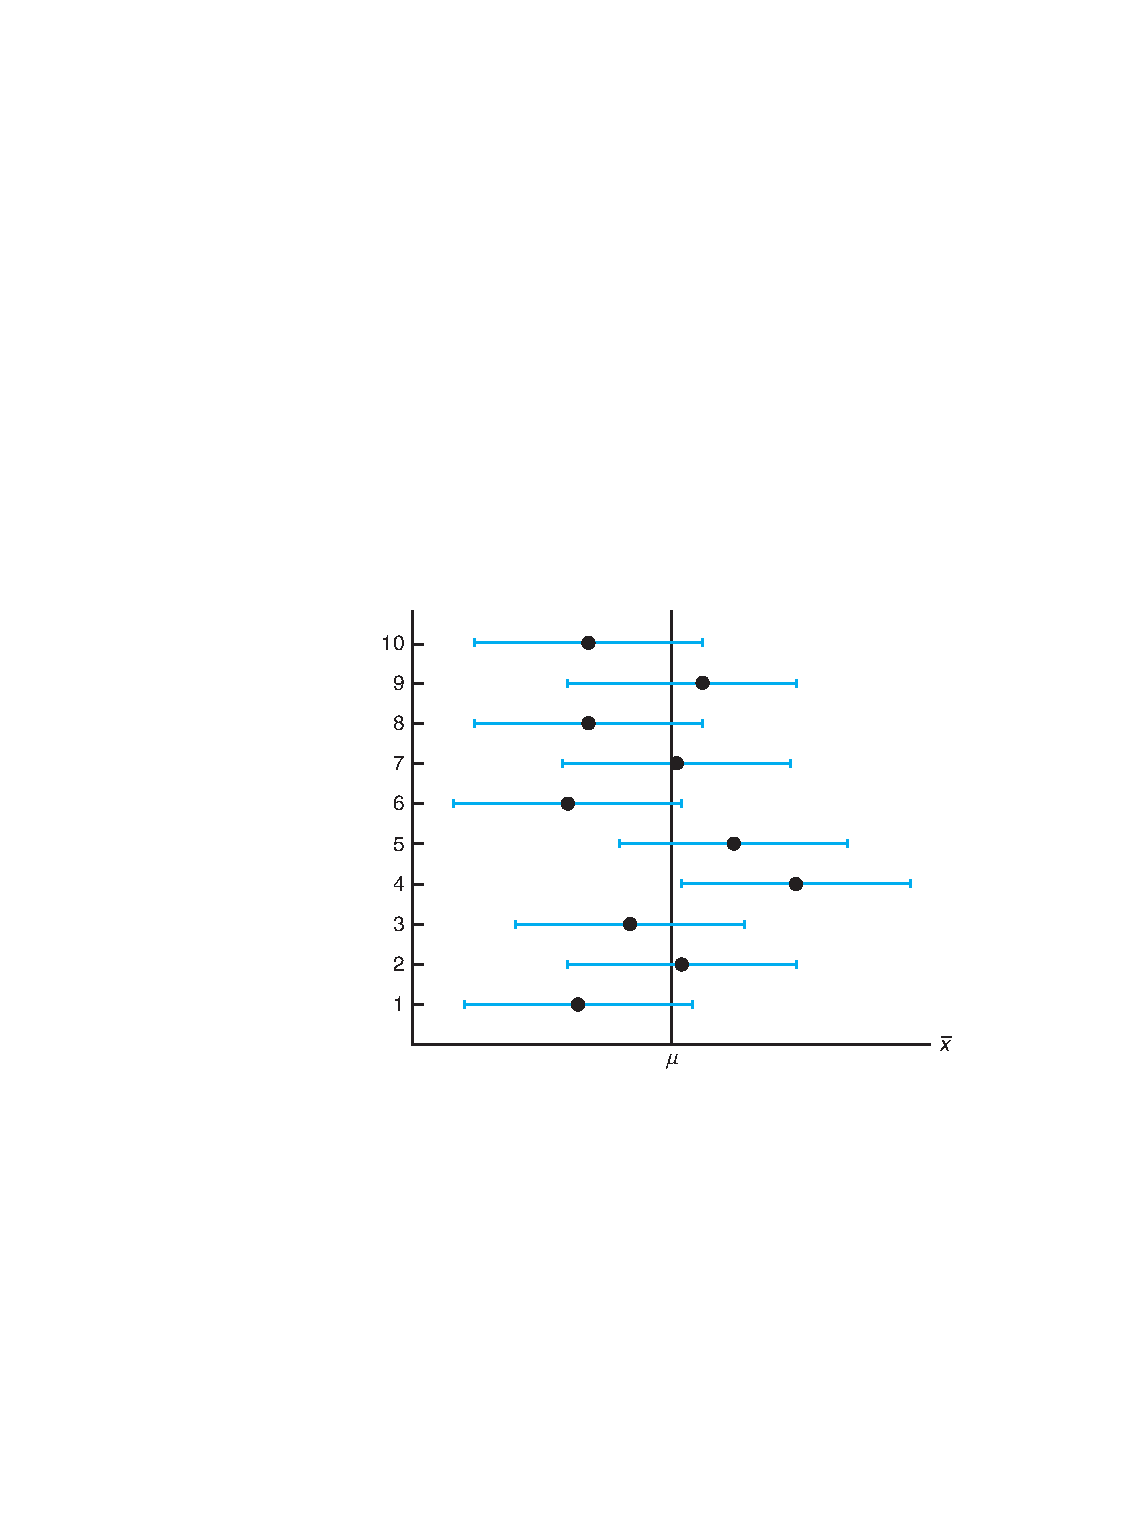
\includegraphics[height=.6\textheight]{img/intervalos}
    \end{center}
  \end{figure}
\end{frame}


\begin{frame}{\color{rosee}IC exacto para $E(X)=\mu$ usando Tchebyshev}\small
Podemos usar Tchebyshev para construir un intervalo para $E(X)$ si $X_i\stackrel{iid}{\sim}$. Por Tcheby para $\overline{X}_n$ y $\eps=\frac{\sigma}{\sqrt{n\alpha}}$ sabemos que:

$$
P\left( \left\vert \overline{X}_{n}-E(X)\right\vert\geq \frac{\sigma}{\sqrt{n\alpha}}\right)\leq \alpha
$$
Entonces 
$$
P\left(  \overline{X}_{n}-\frac{\sigma}{\sqrt{n\alpha}}\leq E(X) \leq  \overline{X}_{n}+\frac{\sigma}{\sqrt{n\alpha}}\right)\geq 1-\alpha
$$
Por lo tanto,
$$
IC_{E(X),\text{Tcheby}}^{(1-\alpha)100\%}=\left[\overline{X}_{n} -\frac{\sigma}{\sqrt{n\alpha}},\overline{X}_{n} + \frac{\sigma}{\sqrt{n\alpha}}\right]
$$

es un intervalo de confianza de nivel $1-\alpha$ para $E(X)$.

\medskip

Notemos que en este caso el IC para $\mu$ no está basado en un estadístico y su distribución (si bien $\overline{X}_n$ es un estimador de $\mu$) sino en la desigualdad de Tcheby. 
\end{frame}


\begin{frame}{\color{rosee} Si $X_i\stackrel{iid}{\sim}$ con $\sigma$ conocida. ¿Cúal $IC_{\mu}^{(1-\alpha)100\%}$ conviene usar?}
\small
\begin{enumerate}
\item Si el modelo estadístico $X_i\stackrel{iid}{\sim} N(\mu,\sigma)$ es \textbf{correcto}, luego 
$$
IC_{\mu, \text{Tcheby}}^{(1-\alpha)100\%}=\left[\overline{X}_{n} -\frac{\sigma}{\sqrt{n\alpha}},\overline{X}_{n} + \frac{\sigma}{\sqrt{n\alpha}}\right]
$$
es mucho más \textbf{ancho} que el intervalo basado en el modelo normal:
$$
IC_{\mu}^{(1-\alpha)100\%}=\left[\overline{X}_{n} - \frac{\sigma}{\sqrt{n}}z_{1-\frac{\alpha}{2}},\overline{X}_{n} + \frac{\sigma}{\sqrt{n}}z_{1-\frac{\alpha}{2}}\right]
$$
\color{gray} para ver esto hay que ver que $\frac{1}{\sqrt{\alpha}}>z_{1-\frac{\alpha}{2}}$. Si bien no vamos a hacer una demostración formal, pruebe, por ejemplo, con $\alpha=0.05$ y $z_{0.975}=1.96$. \color{black}
\item  Si el modelo estadístico $X_i\stackrel{iid}{\sim} N(\mu,\sigma)$ es \textbf{incorrecto}
$$
IC_{\mu, \text{Tcheby}}^{(1-\alpha)100\%}=\left[\overline{X}_{n} -\frac{\sigma}{\sqrt{n\alpha}},\overline{X}_{n} +\frac{\sigma}{\sqrt{n\alpha}}\right]
$$

sigue dando un intervalo de confianza \textbf{exacto} para $\mu$, mientras que $IC_{\mu}^{(1-\alpha)100\%}$ no es un intervalo de confianza \textbf{exacto} \textbf{(será un IC asintótico)} en ese caso.
%sigue funcionando, mientras que el intervalo basado en el modelo normal puede ser un desastre.
\end{enumerate}
\end{frame}

\begin{frame}{\color{rosee} IC para $\sigma^2$ si $X_i\stackrel{iid}{\sim}N(\mu,\sigma^2)$}

    \small Para construir este intervalo de confianza usaremos que si $X_i\stackrel{iid}{\sim}N(\mu,\sigma^2)$ el estadístico $\chi=\frac{(n-1)S^2}{\sigma^2}\sim \chi^2_{n-1}$ tiene distribución chi-cuadrado con $n-1$ grados de libertad. Entonces

    \begin{align*}
       1-\alpha =& P\left(\chi^2_{n-1,\frac{\alpha}{2}}\leq \frac{(n-1)S^2}{\sigma^2}\leq \chi^2_{n-1,1-\frac{\alpha}{2}}\right)\\
       =& P\left(\dfrac{1}{\chi^2_{n-1,1-\frac{\alpha}{2}}}\leq \frac{\sigma^2}{(n-1)S^2}\leq \dfrac{1}{\chi^2_{n-1,\frac{\alpha}{2}}}\right)\\
       =& P\left(\dfrac{(n-1)S^2}{\chi^2_{n-1,1-\frac{\alpha}{2}}}\leq \sigma^2\leq \dfrac{(n-1)S^2}{\chi^2_{n-1,\frac{\alpha}{2}}}\right)
    \end{align*}

    Por lo tanto $IC_{\sigma^2}^{(1-\alpha)100\%}=\left[\dfrac{(n-1)S^2}{\chi^2_{n-1,1-\frac{\alpha}{2}}}, \dfrac{(n-1)S^2}{\chi^2_{n-1,\frac{\alpha}{2}}}\right]$
\end{frame}


\begin{frame}{\color{rosee}IC para $\mu$ si $X_i\stackrel{iid}{\sim}N(\mu,\sigma^2)$ y $\sigma^2$ es desconocida}\small
  \begin{itemize}
  \item Si $\sigma^2$ era conocida para construir el $IC_{\mu}^{(1-\alpha)100\%}$ usamos el \textbf{estadístico}
    \[ Z=\frac{\overline{X}_{n} - \mu}{\sqrt{\frac{\sigma^2}{n}}} \sim
      N(0,1) \]
  \item Si $\sigma^2$ es desconocida para construir el $IC_{\mu}^{(1-\alpha)100\%}$ usaremos el \textbf{estadístico} 
    \[ W=\frac{\overline{X}_{n} - \mu}{\sqrt{\frac{S^2}{n}}} \sim T \] pero no
    sabemos la distribuci\'on $T$ en este caso. Dos opciones:
    \begin{description}
    \item[Opci\'on 1:] buscamos la \textbf{distribuci\'on exacta} $W\sim t_{n-1}$. 
    \item[Opci\'on 2:] buscamos una \textbf{aproximaci\'on asint\'otica} $W\stackrel{D}{\to}N(0,1)$.
  \end{description}
  \end{itemize}
\end{frame}


\begin{frame}{\color{rosee} Distr. exacta de $W$ si $X_i\stackrel{iid}{\sim}N(\mu,\sigma^2)$ y $\sigma^2$ es desconocida}\small
%Nos enfocaremos en las aproximaciones asint\'oticas
 % pero mencionaremos brevemente el caso de la distribuci\'on t-Student.\medskip

Para $X_1,\dots,X_n\stackrel{iid}{\sim}N(\mu,\sigma^2)$%, y $\overline{X}_n$ y $S_n^2$ estimadores de $\mu$ y $\sigma^2$: %respectivamente, luego:
\medskip
\begin{itemize}
\item[(a)] $\overline{X}_n$ e $S_n^2$ son v.a. independientes.\medskip
\item[(b)] $\overline{X}_n\sim N\left(\mu, \frac{\sigma^2}{n}\right)$ y $(n-1)\cdot \frac{S_n^2}{\sigma^2}\sim \chi^2_{n-1}$ 

Llamamos $\chi^2_{n-1}$ a la distribución chi--cuadrado con $n-1$ grados de libertad.\medskip
\item[(c)] Si $Z=\frac{\sqrt{n}(\overline{X}_n-\mu)}{\sigma}\sim N(0,1)$ y $V=(n-1)\cdot \frac{S_n^2}{\sigma^2}\sim\chi^2_{\nu}$ son v.a. \textbf{independientes} entonces la variable $W$
$$ W=\frac{Z}{\sqrt{\frac{V}{\nu}}} \sim T_{\nu}, \text{ t-Student con } \nu \text{  grados de libertad}.$$
%donde $t_{\nu}$ es una t-Student con $\nu$ grados de libertad.
\end{itemize}
Utilizando (a), (b) y (c), se tiene que $ W=\frac{\overline{X}_n-\mu}{\sqrt{\frac{S^2}{n}}}\sim t_{n-1}$.

\end{frame}


 
\begin{frame}{\color{rosee}Distribución t-Student  $\frac{\sqrt{n}(\overline{X}_{n} - \mu)}{S}$ si $X_i\stackrel{iid}{\sim}N(\mu,\sigma^2)$}
\begin{columns}
    \begin{column}[t]{0.48\textwidth}
   \small Distribuci\'on de $W=\frac{\sqrt{n}(\overline{X}_{n} - \mu)}{S}$ para distintos grados de libertad $g=n-1$. A mayor grados de libertad, hay una menor probabilidad de estar a $2$ desvíos estándar de $0$.
  \begin{figure}
    \centering
    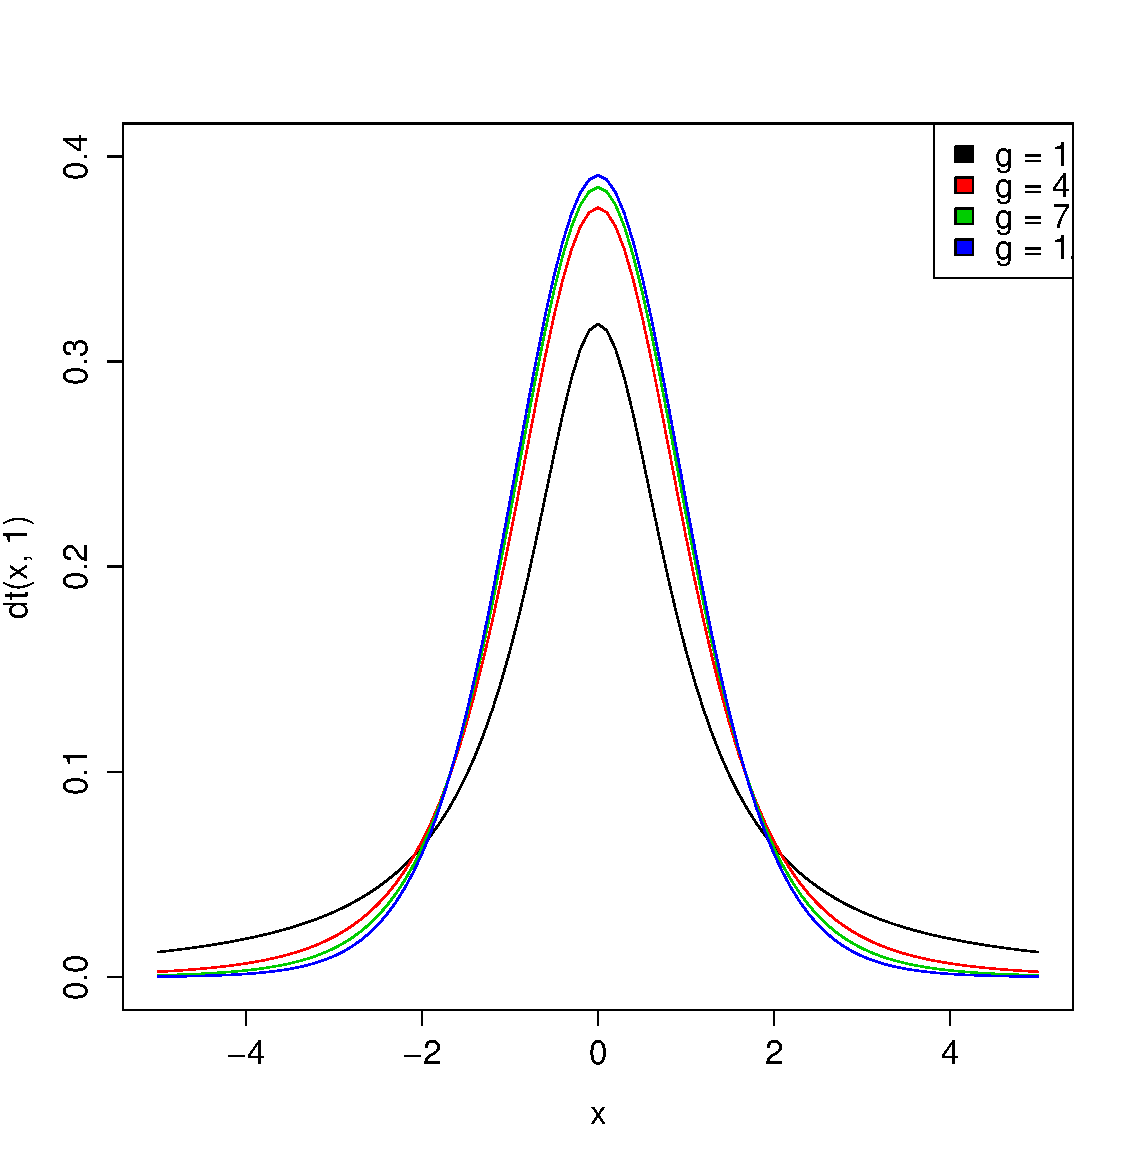
\includegraphics[height=.6\textheight]{img/variast}
  \end{figure}
  \end{column}
    \begin{column}[t]{0.48\textwidth}
  \small  Distribuci\'on de $W=\frac{\sqrt{n}(\overline{X}_{n} - \mu)}{S}$ vs distribución de $\color{red}Z\sim N(0,1) \text { (rojo)}$. La distribución t-Student tiene ``colas más anchas'' porque tiene en cuenta que no se conoce el valor de la varianza de los datos $\sigma^2$.
          \begin{center}
      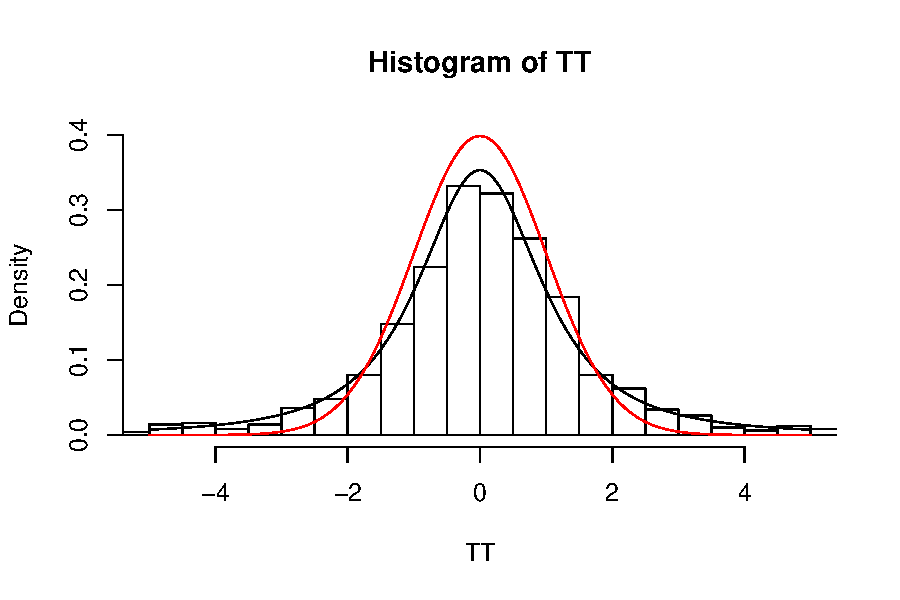
\includegraphics[height=.45\textheight]{img/t-hist}
    \end{center}
  
    \end{column}
  \end{columns}
\end{frame}


 

\begin{frame}{\color{rosee}IC exacto para $\mu$ si $X_i\stackrel{iid}{\sim}N(\mu,\sigma^2)$ y $\sigma^2$ es desconocida} \small
  \begin{itemize}
  \item Si $X_i\stackrel{iid}{\sim}N(\mu, \sigma^2)$ y 
    $\sigma$ es desconocida y si utilizamos el estad\'istico $W$ tiene distribución exacta $t$-Student con $n-1$ grados de libertad
    \[W=\frac{\overline{X}_{n} - \mu}{\frac{S}{\sqrt{n}}}\sim t_{n-1}\]
    \item Entonces el intervalo de confianza
      de $(1-\alpha)100\%$ para $\mu$ est\'a dado por
      \[IC_{\mu}^{(1-\alpha)100\%}=\left[\overline{X}_{n} - t_{1-\frac{\alpha}{2},n-1}\frac{S}{\sqrt{n}} , \overline{X}_{n}
        +t_{1-\frac{\alpha}{2},n-1}\frac{S}{\sqrt{n}}\right]\] donde
      $t_{1-\frac{\alpha}{2},n-1}$ es el cuantil $1-\frac{\alpha}{2}$ de la distribución $t$ de Student con $n-1$ grados de libertad.
  \end{itemize}
    \begin{block}{Interpretaci\'on:}
    Si repetimos muchas veces el experimento de tomar una muestra de
    tama\~no $n$ y hacer el IC del 95\% para $\mu$, aproximadamente el
    95\% de las veces la verdadera media $\mu$ estará contenida en el intervalo estimado (y el 5\% de las veces no!).
  \end{block}
\end{frame}



\begin{frame}{\color{rosee}Ejemplos de ICs exactos para $\mu$ si $X_i\stackrel{iid}{\sim}N(\mu,\sigma^2)$}\small
Se encuestan a $10$ personas para que califiquen un servicio. Asuma que cada calificación $X_i\stackrel{iid}{\sim}N(\mu,\sigma^2)$. La \textbf{media muestral} fue de $\overline{x}_{10} = 2.8$ puntos y la \textbf{desviación muestral} fue de $s_{10} = 0.7$ puntos. Calcule el intervalo de confianza de nivel $90\%$ ($t_{9, 0.05} = 1.833$) para $\mu$.\\~\\

Con $1-\alpha=0.9$ y $n=10$, tenemos que $t_{n-1,\alpha/2 } = t_{9, 0.05} = 1.833$. Entonces: %Usando la fórmula para el intervalo de la slide anterior se tiene que:
$$2.8 - 1.833 \cdot \frac{0.7}{\sqrt{10}} \leq \mu \leq 2.8 + 1.833\cdot \frac{0.7}{\sqrt{10}} .$$

Con un nivel de confianza del $90\%$ esperamos que $\mu$ esté contenida en el intervalo $[2.394;\, 3.206]$. El margen de error es aprox. igual a $0.40575$. 

\textbf{Pregunta}: ¿Qué ocurre con el margen de error del IC si conociéramos que $\sigma = 0.7$?
$$ \text{ Como } \left[2.8 - 1.645 \cdot \frac{0.7}{\sqrt{10}} , 2.8 + 1.645\cdot \frac{0.7}{\sqrt{10}}\right]=[2.43586,3.164136]$$
el margen de error es aproximadamente igual a $0.364$.
\end{frame}



\begin{frame}{\color{rosee}IC exacto para $p$ si $X_i\stackrel{iid}{\sim}Be(p)$ usando Hoeffding} \small
Si $X_i\sim_{iid} Be(p)$ y $\varepsilon>0$ entonces la desigualdad de Hoeffding dice que $$P\left(|\bar{X}_n-p|>\varepsilon\right)\leq 2 e^{-2n\varepsilon^2}$$
Entonces, tomando $\eps=\sqrt{\frac{\ln(2)-\ln(\alpha)}{2n}}=\sqrt{\frac{\ln(2/\alpha)}{2n}}$ vale que $\alpha=2e^{-2n\eps^2}$
$$P\left(\Big\vert\overline{X}_n- p \Big\vert>\sqrt{\frac{\ln(2/\alpha)}{2n}}\right)\leq \alpha$$
Entonces 
$$P\left(\overline{X}_n-\sqrt{\frac{\ln(2/\alpha)}{2n}}\leq p \leq \overline{X}_n+\sqrt{\frac{\ln(2/\alpha)}{2n}}\right)\geq 1-\alpha$$
%    \[IC_{\theta}^{(1-\alpha)100\%}=(\widehat{p}_n-\varepsilon_n,\widehat{p}_n+\varepsilon_n)\]
%    donde
%    \[\varepsilon^2 = \frac{\ln (2/\alpha)}{2n}\]
%    Por la desigualdad de Hoeffding (ver Pr\'actica 1)
 %   obtenemos que para todo $p$ se cumple que
 %   \[P(p \in IC_{\theta}^{(1-\alpha)100\%}) \geq 1- \alpha\] Luego, el intervalo propuesto $IC_{\theta}^{(1-\alpha)100\%}$
 Luego \[IC_{p,\text{Hoeff}}^{(1-\alpha)100\%}=\left[\overline{X}_n-\sqrt{\frac{\ln(2/\alpha)}{2n}}, \overline{X}_n+\sqrt{\frac{\ln(2/\alpha)}{2n}}\right]\]
    es un intervalo de confianza \textbf{exacto} para $p$ de nivel
    $(1-\alpha)100\%$.
   
\end{frame}


\begin{frame}{\color{rosee}IC asint\'oticos para $\mu$ si $X_i\stackrel{iid}{\sim}$ y $p$ si $X_i\stackrel{iid}{\sim}Be(p)$} \small
\textbf{1) Si $X_i\stackrel{iid}{\sim}$ con $\sigma^2$ desconocida}, un $IC_{\mu, \text{ as}}^{(1-\alpha)100\%}$ est\'a dado por
    \[ IC_{\mu,\text{ as}}^{(1-\alpha)100\%}=\left[\overline{X}_{n} -  z_{1-\frac{\alpha}{2}} \frac{S}{\sqrt{n}} , \overline{X}_{n}
      + z_{1-\frac{\alpha}{2}} \frac{S}{\sqrt{n}}
      \right].
    \]

porque $\sqrt{n}\frac{(\overline{X}_n-\mu)}{S}\stackrel{D}{\to}N(0,1)$ por: \textbf{(a)} TCL para $X_i\stackrel{iid}{\sim}$, \textbf{(b)} $\frac{\sigma}{S}\cp 1$, \textbf{(c)} Slutsky aplicado a \textbf{(a)} y \textbf{(b)}. \color{gray} Este es un caso general que permite dar la \textbf{distribución asintótica} del estadístico $W$ en \S12.\color{black}

\bigskip

 \textbf{2) Si $X_i\stackrel{iid}{\sim}Be(p)$, }si $\widehat{p}=\overline{X}_n$, un $IC_{p, \text{ as}}^{(1-\alpha)100\%}$ est\'a dado por
    \[ IC_{p,\text{ as}}^{(1-\alpha)100\%}=\left[ \hat{p}-z_{1-\frac{\alpha}{2}}\sqrt{\frac{\hat{p}(1-\hat{p})}{n}} ,
      \hat{p} + z_{1-\frac{\alpha}{2}}\sqrt{\frac{\hat{p}(1-\hat{p})}{n}}\right]
      \]
porque $\sqrt{n}\frac{(\overline{X}_n-p)}{\sqrt{\widehat{p}(1-\widehat{p})}}\stackrel{D}{\to}N(0,1)$ por: \textbf{(a)} TCL para $X_i\stackrel{iid}{\sim}$, \textbf{(b)} $\frac{\sqrt{p(1-p)}}{\sqrt{\widehat{p}(1-\widehat{p})}}\cp 1$, \textbf{(c)} Slutsky aplicado a \textbf{(a)} y \textbf{(b)}.
\end{frame}

\begin{frame}{\color{rosee}Comentarios sobre $IC_{p, \text{ as}}^{(1-\alpha)100\%}$}
    \begin{itemize}
        \item Si $p\cdot(1-p)\approx 0$ entonces es preferible utilizar el intervalo de confianza para $p$ construido para la desigualdad de Hoeffding.
        \item Por la fórmula del intervalo podría potencialmente pasar que, para algunas muestras el borde inferior del intervalo diera menor que cero o que el borde superior del intervalo diera mayor que uno. 
        \item Por ejemplo, imagine que para ciertos datos muestrales $\munderbar{x}$, se tiene que el intervalo de confianza diera $[-.1,0.3]$. En ese caso, podemos decir que el intervalo de confianza es $[0,0.3]$.
        \item Análogamente imagine que para ciertos datos muestrales $\munderbar{x}$, se tiene que el intervalo de confianza diera $[0.8,1.1]$. En ese caso, podemos decir que el intervalo de confianza es $[0.8,1]$.
       % \item Construir un IC para -\ln(p) y construir a partir de eso un IC para p elevando a e^{-bordes}? 
    \end{itemize}
    
\end{frame}

\begin{frame}{\color{rosee}IC asint\'oticos para $\mu$ si $X_i\stackrel{iid}{\sim}$ y $p$ si $X_i\stackrel{iid}{\sim}Be(p)$} \small

\textbf{Ejercicio 1:} Suponga que tiene $n=300$ datos de cantidad de containers perdidos en distintos puertos de Argentina $X_i\stackrel{iid}{\sim}Poi(\lambda)$. Sabiendo que 
$\displaystyle\sum_{i=1}^{300} x_i=450$ y que $s^2=3$. Encuentre un intervalo de confianza del 95\% para
    la cantidad real de containers perdidos.\color{gray}\[\left[1.5-1.96\cdot \frac{\sqrt{3}}{\sqrt{300}},1.5+1.96\cdot \frac{\sqrt{3}}{\sqrt{300}}\right]=[1.304,1.696]\]\color{black}
\bigskip
  \textbf{Ejercicio 2:}
Sean las variables aleatorias $X_i\stackrel{iid}{\sim} Ber(p)$ que cuentan qué personas están suscriptas a HBO. En una muestra de $n=500$ familias que tienen televisores
    en la ciudad de Hamilton, Canad\'a, se encuentra que $\displaystyle\sum_{i=1}^{500} x_i=340$ est\'an
    suscriptas a HBO. Encuentre un intervalo de confianza del 95\% para
    la proporci\'on real de familias en esta ciudad que est\'an
    suscriptas a HBO.  \color{gray}\[\left[0.68-1.96\cdot \frac{\sqrt{0.68\cdot 0.32}}{\sqrt{500}},0.68+1.96\cdot \frac{\sqrt{0.68\cdot 0.32}}{\sqrt{500}}\right]=[0.639,0.721]\]\color{black}
\end{frame}




\begin{frame}{\color{rosee}IC asint\'oticos basados en estimadores asint. normales} \small
  
    Supongamos ahora más generalmente que $\widehat{\theta}_n$ es un estimador de $\theta$ que es \textbf{asintóticamente normal}, es decir que cumple:
$$
\sqrt{n}\left( \widehat{\theta}_n - \theta\right) \cw N\left(0,V(\theta)\right),
$$
donde $V(\theta)$ es la varianza de la distribución asintótica del estimador $\widehat{\theta}_n$. Supongamos que tenemos un estimador consistente de $V(\theta)$. Por ejemplo, consideremos el estimador \textit{plug-in} $V(\widehat{\theta}_n)$ que es consistente para $V(\theta)$. Entonces, por Slutsky 
$$
\sqrt{n}\frac{\left( \widehat{\theta}_n - \theta\right)}{\sqrt{V(\widehat{\theta}_n)}} \cw N\left(0,1\right),
$$

    Luego, dado un $\alpha > 0$, vale que, cuando $n$ tiende a infinito, vale que:
    \[P\left(-z_{1-\frac{\alpha}{2}} \leq
        \frac{\sqrt{n}(\widehat{\theta}_{n}-\theta)}{\sqrt{V(\widehat{\theta}_n)}} \leq 
        z_{1-\frac{\alpha}{2}}\right) \stackrel{n\to+\infty}{\longrightarrow} 1-\alpha\]


\end{frame}

\begin{frame}{\color{rosee}IC asint\'oticos basados en estimadores asint. normales} 

Por lo tanto, un intervalo de confianza de nivel aproximado $(1-\alpha)100\%$ para $\theta$ basado en el estimador asintóticamente normal $\widehat{\theta}_n$ es 
  \[IC_{\theta, \text{ as}}^{(1-\alpha)100\%}=\left[
  \widehat{\theta}_{n} - z_{1-\frac{\alpha}{2}} \sqrt{\frac{V(\widehat{\theta}_{n})}{n}},\widehat{\theta}_{n} + z_{1-\frac{\alpha}{2}} \sqrt{\frac{V(\widehat{\theta}_{n})}{n}}\right]
  \]

  \bigskip
  
Ejemplos de IC asint\'oticos basados en estimadores asint. normales
  \begin{enumerate}
      \item IC para $\theta$ basado en $\widehat{\theta}_{MV}$
      \item IC para $g(\theta)$ basado en $g(\widehat{\theta}_{MV})$
      \item IC para $P(X\leq x_0)$ en un modelo no paramétrico
      
  \end{enumerate}
\end{frame}

\begin{frame}{\color{rosee}IC asint\'oticos basados en estimadores asint. normales 1}\small
\begin{columns}
  \begin{column}[t]{0.48\textwidth}\color{gray}
        Bajo ciertas \underline{condiciones de regularidad} el estimador de
    m\'axima verosimilitud $\widehat{\theta}_{MV}$ es asint\'oticamente normal:
    \[\sqrt{n} \left(\frac{\widehat{\theta}_{MV}-\theta}
        {\sqrt{[I_1(\theta)]^{-1}}}\right)\cw N\left(0,1\right)\]
  \end{column}
    \begin{column}[t]{0.48\textwidth}
    \color{gray}
       Estimamos a $I_{1}(\theta)$ consistentemente con   el estimador \textit{plug-in} $I_{1}(\widehat{\theta}_{MV})$. Por Slutsky
       \[\sqrt{n} \left(\frac{\widehat{\theta}_{MV}-\theta}
        {\sqrt{[I_{1}(\widehat{\theta}_{MV})]^{-1}}}\right)\cw N\left(0,1\right)\] 
  \end{column}
  \end{columns}
  
  \vspace{12pt}
 Si definimos el intervalo asintótico para $\theta$ de nivel aprox $1-\alpha$ basado en $\widehat{\theta}_{MV}$
    \[IC_{\theta, \text{ as}}^{(1-\alpha)100\%}= \left [\widehat{\theta}_{MV}-z_{1-\frac{\alpha}{2}}
        \sqrt{\frac{I_1\left(\widehat{\theta}_{MV}\right)^{-1}}{n}};
        \widehat{\theta}_{MV}+z_{1-\frac{\alpha}{2}}
        \sqrt{\frac{I_1\left(\widehat{\theta}_{MV}\right)^{-1}}{n}}
      \right]\]
    Entonces vale que 
    $P\left(\theta \in IC_{\theta, \text{ as}}^{(1-\alpha)100\%}\right) \stackrel{n \rightarrow \infty}{\longrightarrow} 1-\alpha$.
  
\end{frame}

\begin{frame}{\color{rosee}IC asint\'oticos basados en estimadores asint. normales 1}\small
  
\textbf{Ejemplo:}  Sean $X_i \stackrel{iid}{\sim} Poi(\lambda)$. El estimador de m\'axima verosimilitud es
    \[\widehat{\lambda}_{MV} = \overline{X}_{n}\]
    y la informaci\'on de Fisher es
    \[I_1(\lambda) = 1/\lambda\]
    entonces el estimador de $I_1(\lambda)$,
    \[I_1(\widehat{\lambda}_{MV}) = 1/\widehat{\lambda}_{MV},\]
    es consistente para $I_1(\lambda)$.
    Luego, un intervalo de confianza de nivel asintótico $(1-\alpha)100\%$ para $\lambda$ basado en $\widehat{\lambda}_{MV}$ es
    \[IC_{\lambda,\text{ as}}^{(1-\alpha)100\%}=\left[\widehat{\lambda}_{MV} - z_{1-\frac{\alpha}{2}} \sqrt{\frac{\widehat{\lambda}_{MV}}{n}},\widehat{\lambda}_{MV} + z_{1-\frac{\alpha}{2}} \sqrt{\frac{\widehat{\lambda}_{MV}}{n}}\right]\]

  
Notemos que ningún estimador asintóticamente normal puede dar lugar a un intervalo de confianza de nivel $(1-\alpha)$ con longitud menor que el que da máxima verosimilitud porque vimos que los estimadores de MV son \textbf{asintóticamente eficientes}.

%Usando máxima verosimilitud, para un mismo nivel dado, obtenemos resultados más precisos, con menos incertidumbre, que con cualquier otro estimador.

\end{frame}



\begin{frame}{\color{rosee}IC asint\'oticos basados en estimadores asint. normales 2}\small

Como el método de MV tiene la propiedad de \textbf{invarianza}, vale que un estimador de $g(\theta)$ es el estimador \textit{plug-in} $g\left(\widehat{\theta}_{MV}\right)$. Es decir, $\widehat{g(\theta)_{MV}}=g\left(\widehat{\theta}_{MV}\right)$.

\medskip

\begin{columns}
  \begin{column}[t]{0.48\textwidth}\color{gray}
        Bajo ciertas \underline{condiciones de regularidad} el estimador de
    m\'axima verosimilitud $g(\widehat{\theta}_{MV})$ es asint\'oticamente normal usando método delta:
    \vspace{12pt}
    
    \scalebox{0.98}{$\sqrt{n} \left(\frac{g(\widehat{\theta}_{MV})-g(\theta)}
        {\sqrt{[I_1(\theta)]^{-1}\cdot g'(\theta)^2}}\right)\cw N\left(0,1\right)$}
  \end{column}
    \begin{column}[t]{0.48\textwidth}
    \color{gray}
       Estimamos a $[I_{1}(\theta)]^{-1}\cdot g'(\theta)^2$ consistentemente con el estimador \textit{plug-in} $[I_{1}(\widehat{\theta}_{MV})]^{-1}\cdot g'(\widehat{\theta}_{MV})^2$. Por Slutsky:
       
       \vspace{12pt}
       
      \scalebox{0.98}{ $\sqrt{n} \left(\frac{g(\widehat{\theta}_{MV})-g(\theta)}
        {\sqrt{[I_{1}(\widehat{\theta}_{MV})]^{-1}\cdot g'(\widehat{\theta}_{MV})^2}}\right)\cw N\left(0,1\right)$ }
  \end{column}
  \end{columns}
  
  \vspace{12pt}
  Si definimos el IC asintótico para $g(\theta)$ de nivel aprox $1-\alpha$ basado en $g(\widehat{\theta}_{MV})$

 \vspace{12pt}
 
    \scalebox{0.85}{$IC_{g(\theta), \text{ as}}^{(1-\alpha)100\%}= \left [g(\widehat{\theta}_{MV})-z_{1-\frac{\alpha}{2}}
        \sqrt{\frac{[I_{1}(\widehat{\theta}_{MV})]^{-1}\cdot g'(\widehat{\theta}_{MV})^2}{n}},
        g(\widehat{\theta}_{MV})+z_{1-\frac{\alpha}{2}}
        \sqrt{\frac{[I_{1}(\widehat{\theta}_{MV})]^{-1}\cdot g'(\widehat{\theta}_{MV})^2}{n}}
      \right]$}

     \vspace{12pt}
     
    Entonces vale que
    $P\left(g(\theta) \in IC_{g(\theta), \text{ as}}^{(1-\alpha)100\%}\right) \stackrel{n \rightarrow \infty}{\longrightarrow} 1-\alpha$.
  
\end{frame}





\begin{frame}{\color{rosee}IC asint\'oticos basados en estimadores asint. normales 2}\small
  \textbf{Ejemplo (a):}
    Dadas $X_i \stackrel{iid}{\sim}Be(p)$ y
    $\psi = g(p) = \ln\left(\frac{p}{1-p}\right)$. La informaci\'on de Fisher de $p$ es
    $I(p)=\frac{1}{p(1-p)}$. 
	Por invarianza, 
    $\widehat{\psi}_{MV}=\ln \left(\frac{\widehat{p}_{MV}}{1-\widehat{p}_{MV}}\right)$. Por el m\'etodo
    delta, la varianza asintótica de $\widehat{\psi}$ es $\frac{1}{p(1-p)}$ que se puede estimar consistentemente usando $
        \frac{1}{\widehat{p}_{MV}(1-\widehat{p}_{MV})}$.
%    \[\widehat{se}(\widehat{\psi}_n)=
%      \frac{1}{\sqrt{n\widehat{p}_n}(1-\widehat{p}_n)}=
%      \sqrt{\frac{\widehat{p}_n(1-\widehat{p}_n)}{n}}\]
    Un intervalo de confianza para $\psi(p)$ basado en $\widehat{\psi}_{MV}$ de nivel aproximado $95\%$ es entonces
    \[ IC_{\psi(p), as}^{95\%}=\left[\widehat{\psi}_{MV} -\frac{1.96}{\sqrt{n \cdot 
          \widehat{p}_{MV}(1-\widehat{p}_{MV})}},\widehat{\psi}_{MV} + \frac{1.96}{\sqrt{n \cdot 
          \widehat{p}_{MV}(1-\widehat{p}_{MV})}}\right]\]

     \textbf{Ejemplo (b):} Dadas $X_i \stackrel{iid}{\sim} N(\mu,\sigma^2)$ con $\mu$
    conocida. Queremos construir un IC para $\ln\sigma$. La
    log-verosimilitud para $\sigma$ es
    \[\ln(\mathcal{L}_{n}(\sigma)) = -n\ln\sigma - \frac{1}{2\sigma^2}\sum_{i=1}^n(X_i-\mu)^2\]

\end{frame}


\begin{frame}{\color{rosee}IC asint\'oticos basados en estimadores asint. normales 2}\small
 \textbf{Ejemplo (b) cont:}  Por lo tanto, el estimador de máxima verosimilitud de $\sigma$ es
    \[\widehat{\sigma}_{MV} = \sqrt{\frac{\sum_{i=1}^n (X_i-\mu)^2}{n}}\]
    
    Buscamos la informaci\'on de Fisher
    \[\dfrac{\partial^2}{\partial \sigma^2}\ln f(X,\sigma)=\frac{1}{\sigma^2} - \frac{3(X-\mu)^2}{\sigma^4}\]
    luego
    \[I_{1}(\sigma) = -\frac{1}{\sigma^2} + \frac{3E\left[ (X-\mu)^2 \right]}{\sigma^4} =
      \frac{2}{\sigma^2}\]

Por invarianza, 
    $\widehat{\psi}_{MV} =\ln\widehat{\sigma}_{MV}$. Por el método delta, 
    \[\sqrt{n}\left(\widehat{\psi}-\psi\right)\stackrel{D}{\to} N\left(0,\frac{\sigma^{2}}{2} \frac{1}{\sigma^{2}}\right)=N\left(0, \frac{1}{2}\right)\]

Luego, un intervalo de confianza para $\psi$ basado en $\widehat{\psi}_{MV}$ de nivel aproximado $95\%$ es
      \[IC_{\psi, \text{ as}}^{95\%}=\left[\widehat{\psi}_n -\frac{1.96}{\sqrt{2n}},\widehat{\psi}_n + \frac{1.96}{\sqrt{2n}}\right]\]
  
\end{frame}

\begin{frame}{\color{rosee}IC asint\'oticos basados en estimadores asint. normales 3}\small
Sean $X_i\stackrel{iid}{\sim}$, supongamos que queremos construir un IC para $F(x_{0})=P(X\leq x_{0})$. ¿Cómo construimos $IC_{P(X\leq x_0),\text{ as}}^{95\%}$? En primer lugar, un estimador del parámetro $F(x_0)=P(X\leq x_0)$ es \[\widehat{F}_n(x_0) = \frac{1}{n} \sum_{i=1}^n I(X_i \leq x_0)\]
 Notemos que $I(X_{i}\leq x_0)\stackrel{iid}{\sim} Ber(F(x_{0}))$. $\widehat{F}_n(x)$ es simplemente la media muestral de la muestra aleatoria $I(X_1 \leq x),\dots,I(X_n \leq x)$. Entonces:  \[ \color{dodgerblue}E(\widehat{F}_n(x)) = F(x), \quad \color{rosee}Var(\widehat{F}_n(x)) = \frac{F(x)(1-F(x))}{n}, \quad \color{orang}\widehat{F}_n(x) \cp F(x)\]   
Por lo tanto, \[\scalebox{0.95}{$
IC_{F(x_0),\text{ as}}^{95\%}=\left[\widehat{F}_{n}(x_0) -1.96\sqrt{\frac{\widehat{F}_{n}(x_0)(1-\widehat{F}_{n}(x_0))}{n}},\widehat{F}_{n}(x_0) + 1.96\sqrt{\frac{\widehat{F}_{n}(x_0)(1-\widehat{F}_{n}(x_0))}{n}}\right]
$}\]

es un intervalo de confianza de nivel asintótico 95\% para $F(x_0)$.

\end{frame}


\begin{frame}{\color{rosee}IC puntuales vs IC uniformes}
\small
\begin{itemize}
   % \item Otra categoría en la que clasificamos los intervalos de confianza es si son IC puntuales o IC uniformes.

\item Los IC \textbf{puntuales} tienen un margen de error que depende de algún \textbf{parámetro conocido} o cuyo margen de error es \textbf{aleatorio}. 

\item Los IC \textbf{uniformes} tienen un margen de error que no depende de ningún \textbf{parámetro conocido ni de la distribución de los datos} y que para cualquier valor del parámetro $\theta$ el margen de error es el mismo.

\item Ejemplo 1 de un IC uniforme: si $X_i\stackrel{iid}{\sim}Be(p)$ el IC para $p$ construido por la desigualdad de Hoeffding.

\item Ejemplo 2 de un IC uniforme: si $X_i\stackrel{iid}{\sim}N(\mu,\sigma^2)$ con $\mu$ conocida el IC para $\ln(\sigma)$ construido a partir del estimador de MV.

\item Otro ejemplo de un intervalo de confianza uniforme para $p$ si $X_i\stackrel{iid}{\sim}Be(p)$ es \textbf{acotando el margen de error} del intervalo de la slide \S17 ya que $\widehat{p}(1-\widehat{p})\leq 0.25$, por lo tanto: 
\[IC_{p,\text{ as, unif}}^{(1-\alpha)100\%}=\left[ \hat{p}-z_{1-\frac{\alpha}{2}}\sqrt{\frac{0.25}{n}} ,
      \hat{p} + z_{1-\frac{\alpha}{2}}\sqrt{\frac{0.25}{n}}\right]\]
\end{itemize}
  %  Hablar del margen de error, categorizar los ICs anteriores en estas dos categorias y construir el IC uniforme para el caso Bernoulli
\end{frame}
%\begin{frame}{\color{rosee}Intervalo de confianza para una estimaci\'on no param\'etrica} \small
%  \begin{block}{Desigualdad de Dvoretzky-Kiefer-Wolfowitz (DKW)}
%    Dadas $X_1,\dots,X_n \sim F$ para cualquier $\varepsilon > 0$
%    \[P\left(\sup_{x} |F(x)-\widehat{F}_n(x)| > \varepsilon \right) \leq 2e^{-2n\varepsilon^2}\]
%  \end{block}
%  \begin{block}{IC no param\'etrico de nivel $1-\alpha$ para $F$}
%    Definimos
%    \[L(x) = \max \left\{\widehat{F}_n(x) -\varepsilon_n,0 \right\}
%      \quad\mbox{y}\quad U(x) = \min \left\{\widehat{F}_n(x) +\varepsilon_n,1
%      \right\}\] donde
%    \[\varepsilon_n = \sqrt{\frac{1}{2n}\ln\left (\frac{2}{\alpha}\right )}\]
%    Por la desigualdad DKW tenemos que para cualquier $F$
%    \[P\left(L(x) \leq F(x) \leq U(x) \;\mbox{para todo $x$}\right) \geq 1-\alpha\]
%  \end{block}
%\end{frame}
%
%\begin{frame}{\color{rosee}Intervalo de confianza para una estimaci\'on no
%    param\'etrica} \small
%  \begin{exampleblock}{Ejemplo}
%    Cox y Lewis (1966) reportaron 799 tiempos de espera entre pulsos
%    sucesivos a lo largo de una fibra nerviosa.
%    % La Figura muestra la
%    % funci\'on de distribuci\'on acumulada emp\'irica. Los datos de la
%    % muestra se indican con los segmentos verticales en el eje $x$.
%
%    \medskip Supongamos que queremos estimar la probabilidad de que un
%    tiempo de espera est\'e entre $0.4$ y $0.6$ segundos. La
%    estimaci\'on puntual es
%    \[\widehat{F}_n(0.6)-\widehat{F}_n(0.4)= 0.93-0.84=0.09\,.\]
%    Las l\'ineas punteadas dan un IC de nivel $95\%$ usando
%    \[\varepsilon = \sqrt{log(2/0.05)/2n}=0.48\,.\]
%  \end{exampleblock}
%\end{frame}
%
%\begin{frame}{\color{rosee}Intervalo de confianza para una estimaci\'on no
%    param\'etrica} \small
%  \begin{figure}
%    \centering
%    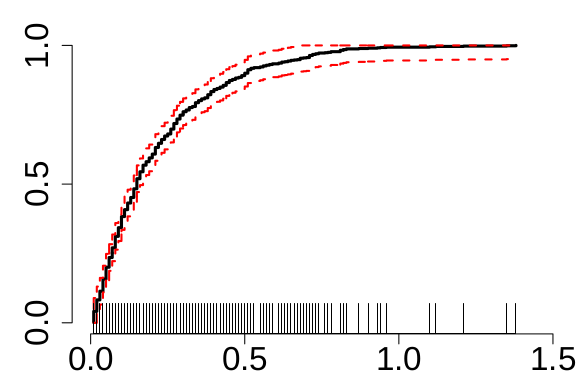
\includegraphics[height=.8\textheight]{img/nerv.png}
%  \end{figure}
%\end{frame}
%
%
%\begin{frame}{\color{rosee}Intervalo de predicci\'on} \small
%  \begin{exampleblock}{Ejemplo (panchos)}
%    Consideramos la siguiente muestra de porcentaje de contenido graso
%    de $n = 10$ panchos elegidos al azar (``Sensory and Mechanical
%    Assessment of the Quality of Frank-furters,'' J. Texture Stud.,
%    1990: 395–409)
%    \[25.2\quad21.3\quad22.8\quad17.0\quad29.8\quad21.0\quad25.5\quad16.0\quad20.9\quad19.5\]
%    Supongamos que fueron elegido de una distribuci\'on normal, un
%    intervalo de confianza de nivel $95\%$ para la media poblacional de
%    porcentaje de contenido graso es
%    \[ \overline{x} \pm t_{0.025,9} \frac{s}{\sqrt{n}} = 21.90 \pm 2.96
%      = (18.94; 24.86)\] Sin embargo, si queremos comer un solo pancho
%    de este tipo queremos una predicci\'on del contenido graso. La
%    predicci\'on puntual, an\'alogamente la estimaci\'on puntual es solo
%    $\overline{x} = 21.90$. No da informaci\'on sobre la precisi\'on.
%  \end{exampleblock}
%\end{frame}
%
%\begin{frame}{\color{rosee}Intervalo de predicci\'on}\small
%  Dada una muestra aleatoria $X_1,X_2,\dots,X_n$ queremos predecir
%  $X_{n+1}$. Una estimaci\'on puntual es $\overline{X}_{n}$. El error de
%  predicci\'on (aleatorio) es
%  \[\overline{X}_{n}-X_{n+1}\,.\]
%  Su esperanza
%  \[E\left(\overline{X}_{n}-X_{n+1}\right) = E\left(\overline{X}_{n}\right)
%    -E\left(X_{n+1}\right) = \mu-\mu = 0\]
%  Como $X_{n+1}$ es
%  independiente de $X_1,\dots,X_n$, es independiente tambi\'en de
%  $\overline{X}_n$, luego la varianza del error de predicci\'on es:
%  \[Var\left(\overline{X}_{n} - X_{n+1} \right) =
%    Var\left(\overline{X}_{n}\right) + Var\left(X_{n+1}\right) = Var(X)
%    \left(\frac{1}{n}+1\right)\] 
%\end{frame}
%
%\begin{frame}{\color{rosee}Intervalo de predicci\'on}\small
%  El error de predicci\'on es una combinaci\'on lineal de variables
%  aleatorias normales e independientes, luego tambi\'en es normal:
%  \[Z =
%    \frac{\left(\overline{X}_{n}-X_{n+1}\right)-0}{\sqrt{\sigma^2\left(\frac{1}{n}+1\right)}}
%    =
%    \frac{\overline{X}_{n}-X_{n+1}}{\sqrt{\sigma^2\left(\frac{1}{n}+1\right)}}
%    \sim N(0,1)\]
%  \begin{block}{Intervalo de predicci\'on}
%    Un intervalo de predicc\'ion para una nueva observaci\'on generada
%    por una distribuci\'on normal es
%    \[\overline{x} \pm t_{\alpha/2, n-1} s \sqrt{1+\frac{1}{n}}\]
%    El nivel de predicci\'on es $(1-\alpha)100\%$.
%  \end{block}
%\end{frame}
%
%\begin{frame}{\color{rosee}Intervalo de predicci\'on}
%  \begin{block}{Interpretaci\'on}
%    La interpretaci\'on del nivel de predicci\'on $95\%$ es similar a la
%    del nivel de confianza $95\%$. Si el intervalo
%    \[\overline{x} \pm t_{\alpha/2, n-1} s \sqrt{1+\frac{1}{n}}\]
%    se calcula para muchas muestras, a la larga, el $95\%$ de esos
%    intervalos incluir\'an al nuevo valor de $X$
%  \end{block}
%\end{frame}
%
%\begin{frame}{\color{rosee}Intervalo de predicci\'on}\small
%  \begin{exampleblock}{Ejempo (panchos)}
%    Con $n=10$, $x=21.90$, $s=4.134$ y $t_{0.025,9}=2.262$, un intervalo
%    de predicci\'onp para el contenido grado de un pancho es
%    \[21.90 \pm 2.262 \cdot 4.134 \cdot \sqrt{1+\frac{1}{10}} = 21.90
%      \pm 9.81 = (12.09;31.71)\] Este intervalo es bastante ancho,
%    indicando incerteza sobre el contenido graso. Notemos que el ancho
%    del intervalo predictivo es m\'as del triple que el intervalo de confianza.
%  \end{exampleblock}
%\end{frame}
%
%\begin{frame}{\color{rosee}Intervalo de predicci\'on}\small
%  \begin{block}{Predicci\'on vs confianza}
%    El \textbf{error de predicci\'on} es una resta de dos variables
%    aleatorias
%    \[\overline{X}_{n} - X_{n+1}\]
%    mientras que el \textbf{error de estimaci\'on} es la diferencia
%    entre una variable aleatoria de un valor fijo pero desconocido.
%    \[\overline{X}_{n} - \mu\]
%    El intervalo de predicci\'on es m\'as ancho que el intervalo de
%    confianza porque hay m\'as variabilidad en el error de predicci\'on
%    (debido a $X_{n+1}$) que en el error de estimaci\'on.
%
%    \bigskip De hecho, cuando $n \rightarrow \infty$ el intervalo de
%    confianza se reduce a $\mu$ mientras que el intervalo de
%    predicci\'on a $\mu \pm z_{\alpha/2} \sigma$.
%  \end{block}
%\end{frame}

%
%\begin{frame}{\color{rosee}Bootstrap} \small
%  \begin{block}{Bootstrap}
%    La t\'ecnica \textbf{bootstrap}, desarrollada por Bradley Efron en
%    1979, nos permite calcular un intervalo de confianza cuando la
%    poblaci\'on no es normal pero el tama\~no de muestra no es grande.
%  \end{block}
%
%  \begin{exampleblock}{Ejemplo}
%    Cuando estudiamos la varianza de un estimador la mencionamos como
%    una t\'ecnica para estimar errores est\'andar.
%
%    \bigskip Repasemos la idea con un ejemplo.
%  \end{exampleblock}
%  % \item ¿C\'omo hallamos intervalos de confianza para otros
%  %   par\'ametros
%  %   como alg\'un percentil de la distribuci\'on poblacional?
%\end{frame}
%
%\begin{frame}{\color{rosee}Bootstrap}\small
% \begin{exampleblock}{Ejemplo (propinas)}
%   Queremos estudiar el porcentaje de propina que recibe el personal de
%   cierta empresa de delivery:
%   \begin{align*}
%     22.7&\quad 16.3\quad 13.6\quad 16.8\quad 29.9\quad 15.9\quad
%           14.0\quad 15.0\quad 14.1\quad 18.1\quad\\
%     22.8&\quad 27.6\quad 16.4\quad 16.1\quad 19.0\quad 13.5\quad
%           18.9\quad 20.2\quad 19.7\quad 18.2\quad\\
%     15.4&\quad 15.7\quad 19.0\quad 11.5\quad 18.4\quad 16.0\quad
%           16.9\quad 12.0\quad 40.1\quad 19.2
%   \end{align*}
%   Buscamos un intervalo de confianza para la media poblacional del
%   porcentaje de propina.
%   \begin{itemize}
%   \item La distribución de la variable parece
%     asim\'etrica: la mayor\'ia de las propinas est\'an entre $10\%$ y
%     $20\%$ pero algunas propinas grandes rompen la simetr\'ia (y la
%     posibilidad de suponer normalidad)
%   \end{itemize}
% \end{exampleblock}
%\end{frame}
%
%\begin{frame}{\color{rosee}Bootstrap}\small
%  \begin{exampleblock}{Ejemplo (propinas)}
%    \begin{figure}
%      \centering
%      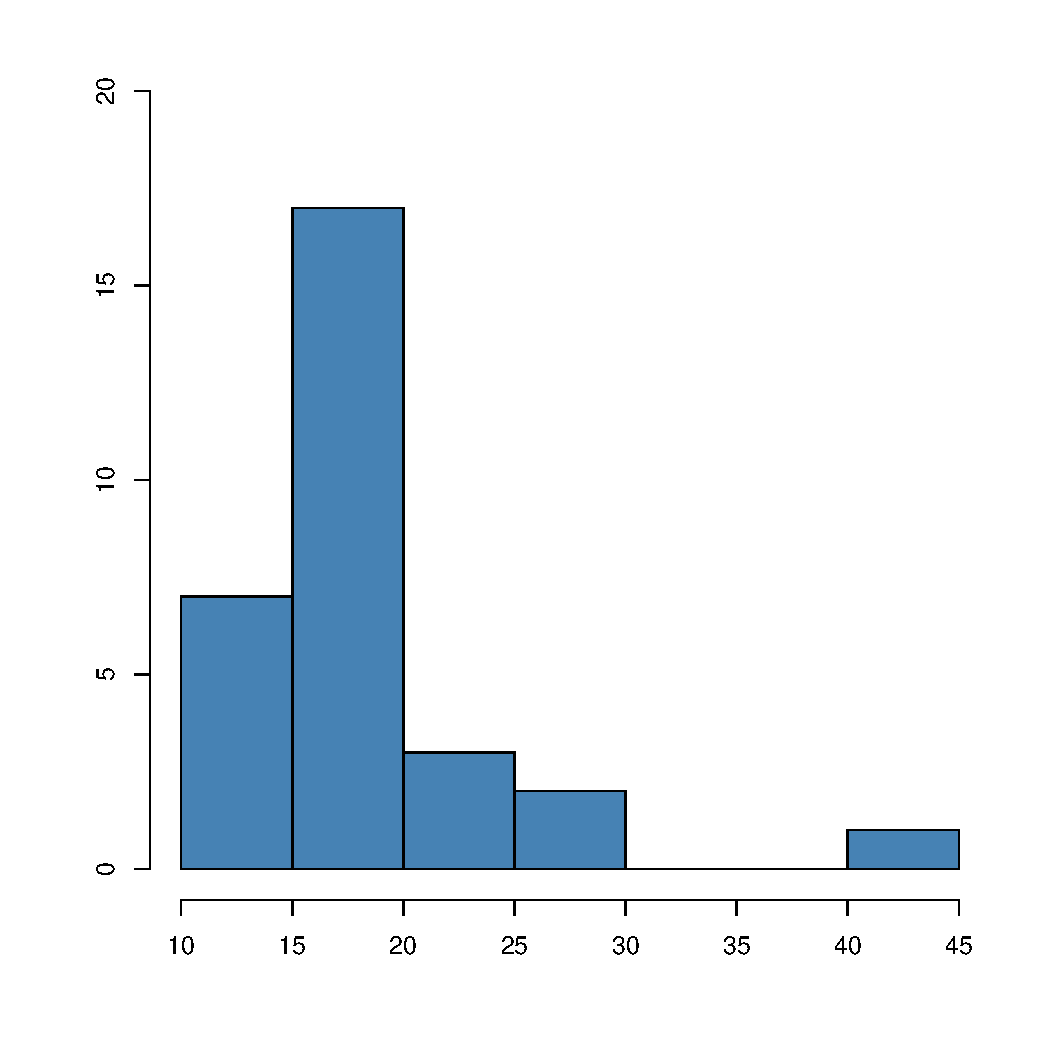
\includegraphics[height=.8\textheight]{img/hist-tips.pdf}
%    \end{figure}
%  \end{exampleblock}
%\end{frame}
%
%\begin{frame}{\color{rosee}Bootstrap} \small
% \begin{exampleblock}{Ejemplo (propinas)}
%   Consideramos nuestras $30$ observaciones como una poblaci\'on:
%   \begin{itemize}
%   \item Tomamos muchas ($N=999$) muestras de tama\~no $30$ con
%     reemplazo (si no ser\'ian todas iguales!).
%   \item Calculamos nuestro estimador para cada muestra obteniendo
%     $N=999$ estimaciones.
%   \item Definimos $s_{boot}$ como el desv\'io est\'andar de las
%     $N=999$ estimaciones bootstrap:
%     \[s_{boot}^2= \frac{1}{999-1} \sum_{i=1}^n (\overline{x_i}^* -
%       \overline{X}_{n}^*)^2\]
%   \end{itemize}
% \end{exampleblock}
%\end{frame}
%
%\begin{frame}{\color{rosee}Bootstrap}\small
%  \begin{exampleblock}{Ejemplo (propinas)}
%    \begin{figure}
%      \centering
%      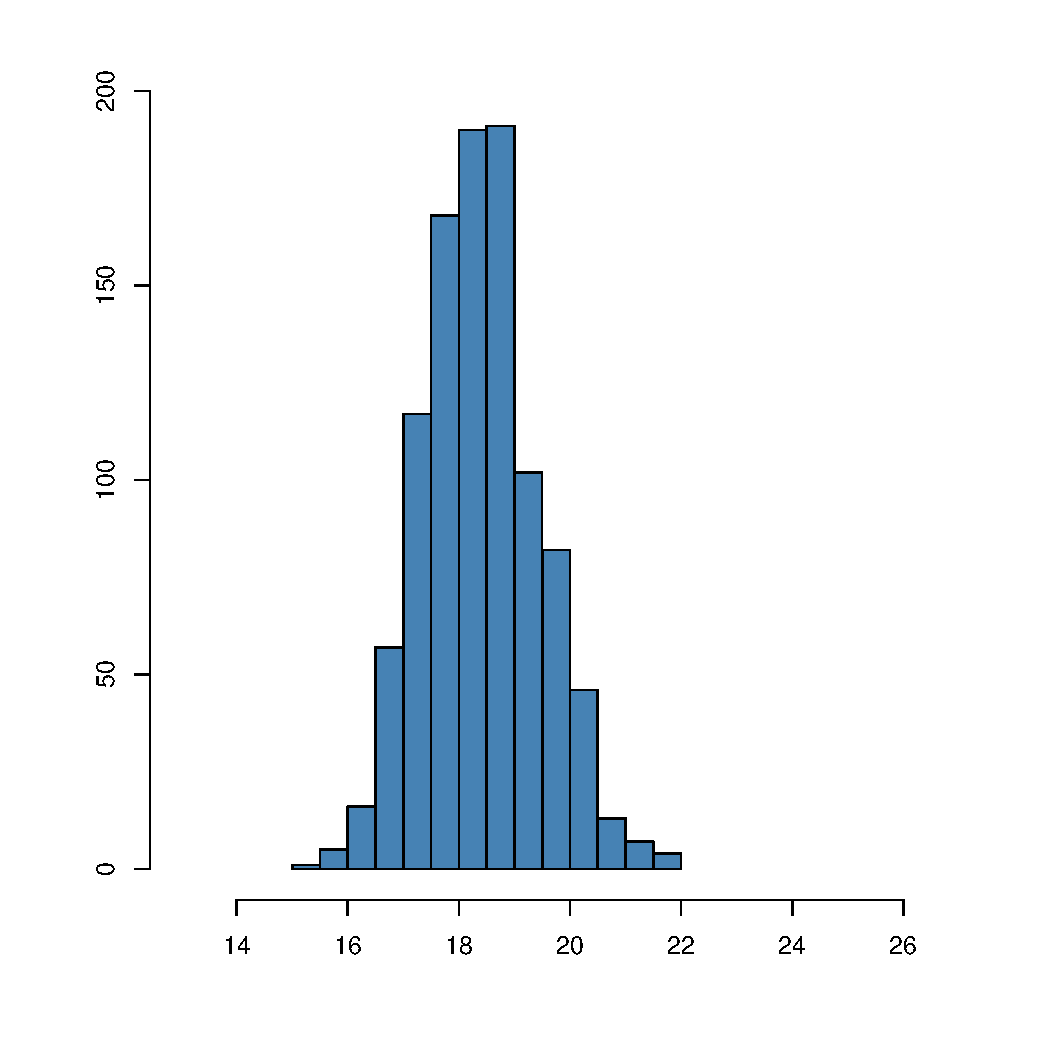
\includegraphics[height=.8\textheight]{img/hist-tips-boot.pdf}
%    \end{figure}
%  \end{exampleblock}
%\end{frame}
%
%% \begin{frame}{\color{rosee}Bootstrap}\small
%%   \begin{exampleblock}
%%     Si supusi\'eramos normalidad podr\'iamos calcular un intervalo de
%%     confianza de nivel $95\%$ como
%%     \[\left(\overline{X}_{n} - z_{0.025} s_{boot}, \overline{X}_{n} +
%%         z_{0.025} s_{boot}\right)\]
%%   \end{exampleblock}
%% \end{frame}
%
%\begin{frame}{\color{rosee}Bootstrap} \small
%%  \begin{block}{Distribuci\'on emp\'irica}
%%    La \textbf{distribuci\'on emp\'irica de los datos} es la
%%    distribuci\'on de la poblaci\'on conformada exclusivamente por los
%%    datos de la muestra obtenida.
%%  \end{block}
%  \begin{exampleblock}{Ejemplo}
%    Elegimos al azar $10$ n\'umeros enteros entre $1$ y $8$:
%    \[1 \quad 1 \quad 2 \quad 3 \quad 3 \quad 3 \quad 3 \quad 4 \quad 7
%      \quad 7\] La distribuci\'on emp\'irica es
%    \begin{table}
%      \centering
%      \begin{tabular}{|c|ccccc|}
%        \hline
%        x & 1 & 2 & 3 & 4 & 7\\
%        p(x) & 2/10 & 1/10 & 4/10 & 1/10 & 2/10\\
%        \hline
%      \end{tabular}
%    \end{table}
%  \end{exampleblock}
%\end{frame}
%
%\begin{frame}{\color{rosee}Bootstrap} \small
%    \begin{block}{Notaci\'on}
%    Si llamamos $F$ a la distribuci\'on de la cual provienen los datos,
%    llamamos $\widehat{F}_{n}$ a la distribuci\'on emp\'irica de los datos.
%  \end{block}
%  \begin{exampleblock}{Ejemplo (cont.)}
%    En el ejemplo anterior $F$ y $\widehat{F}_{n}$ son:
%    \begin{table}
%      \centering
%      \setlength{\tabcolsep}{4pt}
%      \begin{tabular}{|c|cccccccc|}
%        \hline
%        $x$                      & 1    & 2    & 3    & 4    & 5   & 6   & 7    & 8   \\
%        \mbox{verdadera} $p(x)$  & 1/8  & 1/8  & 1/8  & 1/8  & 1/8 & 1/8 & 1/8  & 1/8 \\
%        \mbox{emp\'irica} $p(x)$ & 2/10 & 1/10 & 4/10 & 1/10 & \textbf{0}   & \textbf{0}   & 2/10 & \textbf{0}   \\
%        \hline
%      \end{tabular}
%    \end{table}
%  \end{exampleblock}
%  \begin{alertblock}{Observaci\'on}
%    Siempre conocemos $\widehat{F}_{n}$ expl\'icitamente. En particular, el
%    valor esperado de $\widehat{F}_{n}$ es la media muestral $\overline{x}$
%    (¿por qu\'e?).
%  \end{alertblock}
%
%\end{frame}
%
%\begin{frame}{\color{rosee}Bootstrap}
%  \begin{block}{Muestra bootstrap}
%    Supongamos que tenemos $n$ observaciones
%    \[x_1, x_2, \dots, x_n\] que provienen de una distribuci\'on $F$.
%
%    \bigskip Una \textbf{muestra bootstrap} es una nueva muestra del
%    mismo tama\~no extraida con reposici\'on de la muestra original.
%
%    \bigskip Es decir, tomamos una muestra de tama\~no $n$ de la
%    distribuci\'on emp\'irica $\widehat{F}_{n}$.
%  \end{block}
%
%\end{frame}
%
%\begin{frame}{\color{rosee}Bootstrap} \small
%  \begin{block}{}
%    \begin{enumerate}
%    \item $x_1, x_2, \dots, x_n$ es una muestra que proviene de la
%      distribuci\'on $F$.
%    \item $\widehat{\theta}_{n}$ es un estimador calculado para esa muestra.
%    \item $\widehat{F}_{n}$ es la distribuci\'on emp\'irica de los datos.
%    \item $x_1^*, x_2^*, \dots, x_n^*$ es una muestra bootstrap (mismo
%      tama\~no).
%    \item $\theta^{\ast}_{n}$ es el estimador calculado para la nueva muestra.
%    \end{enumerate}
%  \end{block}
%  \begin{block}{}
%    La idea detr\'as de bootstrap es que
%    \begin{enumerate}
%    \item $\widehat{F}_{n} \approx F$.
%    \item \textbf{Si el tamaño de muestra es grande}, la distribución de $\widehat{\theta}_{n}$ se puede aproximar por la distribución de
%      $\theta^{\ast}_{n}$. El Bootstrap es un técnica que tiene validez \textbf{asintótica}.
%    \end{enumerate}
%  \end{block}
%\end{frame}
%
%\begin{frame}{\color{rosee}Bootstrap} \small
%  \begin{exampleblock}{Ejemplo}
%    A partir de la siguiente muestra queremos estimar la media $\mu$ de
%    la distribuci\'on y dar un intervalo de confianza de nivel $80\%$:
%    \[30 \quad 37 \quad 36 \quad 43 \quad 42 \quad 43 \quad 43 \quad 46
%      \quad 41 \quad 42\]
%    La media muestral es
%    \[\overline{x} = 40.3 \,.\]
%    Para construir el intervalo de confianza necesitamos saber c\'omo
%    var\'ia la distribuci\'on de $X$ alrededor de $\mu$. Queremos
%    conocer la distribuci\'on de
%    \[ \Delta = \overline{X}_{n} - \mu\]
%  \end{exampleblock}
%\end{frame}
%
%\begin{frame}{\color{rosee}Bootstrap} \small
%  \begin{exampleblock}{Ejemplo}
%    Si la conoci\'eramos podr\'iamos calcular $\delta_{0.1}$ y $\delta_{0.9}$, los cuantiles $0.1$ y $0.9$ de $\Delta$ y hacer
%    \[P\left (\delta_{0.1} \leq \overline{X}_{n} - \mu \leq \delta_{0.9} \right) =
%      0.8 \Leftrightarrow P(\overline{X}_{n} - \delta_{0.1} \geq \mu \geq
%      \overline{X}_{n} - \delta_{0.9}) = 0.8\] lo que dar\'ia un intervalo
%    de confianza de nivel $80\%$:
%    \[\left [ \overline{X}_{n} - \delta_{0.9}, \overline{X}_{n} - \delta_{0.1} \right]\]
%  \end{exampleblock}
%\end{frame}
%
%\begin{frame}{\color{rosee}Bootstrap} \small
%  \begin{exampleblock}{Ejemplo}
%    Generamos $20$ muestras bootstrap, cada una de tama\~no $10$.
%    \scriptsize
%    \setlength{\tabcolsep}{3.5pt}
%    \begin{table}
%      \begin{tabular}{cccccccccccccccccccc}
%        43 & 36 & 46 & 30 & 43 & 43 & 43 & 37 & 42 & 42 & 43 & 37 & 36 & 42 & 43 & 43 & 42 & 43 & 42 & 43 \\
%        43 & 41 & 37 & 37 & 43 & 43 & 46 & 36 & 41 & 43 & 43 & 42 & 41 & 43 & 46 & 36 & 43 & 43    & 43 & 42 \\ 
%        42 & 43 & 37 & 43 & 46 & 37 & 36 & 41 & 36 & 43 & 41 & 36 & 37 & 30 & 46 & 46 & 42 & 36    & 36 & 43 \\  
%        37 & 42 & 43 & 41 & 41 & 42 & 36 & 42 & 42 & 43 & 42 & 43 & 41 & 43 & 36 & 43 & 43 & 41    & 42 & 46 \\  
%        42 & 36 & 43 & 43 & 42 & 37 & 42 & 42 & 42 & 46 & 30 & 43 & 36 & 43 & 43 & 42 & 37 & 36    & 42 & 30 \\  
%        36 & 36 & 42 & 42 & 36 & 36 & 43 & 41 & 30 & 42 & 37 & 43 & 41 & 41 & 43 & 43 & 42 & 46    & 43 & 37 \\  
%        43 & 37 & 41 & 43 & 41 & 42 & 43 & 46 & 46 & 36 & 43 & 42 & 43 & 30 & 41 & 46 & 43 & 46    & 30 & 43 \\  
%        41 & 42 & 30 & 42 & 37 & 43 & 43 & 42 & 43 & 43 & 46 & 43 & 30 & 42 & 30 & 42 & 30 & 43    & 43 & 42 \\  
%        46 & 42 & 42 & 43 & 41 & 42 & 30 & 37 & 30 & 42 & 43 & 42 & 43 & 37 & 37 & 37 & 42 & 43    & 43 & 46 \\  
%        42 & 43 & 43 & 41 & 42 & 36 & 43 & 30 & 37 & 43 & 42 & 43 & 41 & 36 & 37 & 41 & 43 & 42    & 43 & 43 
%      \end{tabular}
%    \end{table}
%    \small
%    Calculamos $\delta^* = \overline{x}^* - \overline{x}$ para cada
%    muestra (cada columna) y los ordenamos de menor a mayor:
%    \begin{align*}
%      -1.6 & \;,\; -1.4\;,\;-1.4\;,\;-0.9\;,\;-0.5 \;,\; -0.2 \;,\; -0.1 \;,\; 0.1 \;,\; 0.2\;,\; 0.2 \;,\; 0.4 \;,\;\\
%      0.4 & \;,\; 0.7 \;,\; 0.9 \;,\; 1.1 \;,\; 1.2\;,\; 1.2 \;,\; 1.6 \;,\; 1.6 \;,\; 2.0
%    \end{align*} 
%  \end{exampleblock}
%\end{frame}
%
%\begin{frame}{\color{rosee}Bootstrap} \small
%  \begin{exampleblock}{Ejemplo}
%    Aproximamos los valores $\delta_{0.1}$ y $\delta_{0.9}$ por
%    $\delta^*_{0.1}$ y $\delta^*_{0.9}$.
%
%    \bigskip Como $\delta^*_{0.9}$ es el percentil $90$ elegimos el
%    elemento de la posici\'on $18$: $1.6$.  An\'alogamente, como
%    $\delta^*_{0.1}$ es el percentil $10$ elegimos el elemento de la
%    posici\'on $2$: $-1.4$.
%
%    \bigskip Luego, el intervalo de confianza bootstrap de nivel $80\%$
%    para $\mu$ es
%    \[\left [ \overline{x}-\delta^*_{0.9} \;;\; \overline{x} - \delta^*_{0.1} \right] = \left
%        [40.3 -1.6 \;;\; 40.3 + 1.4 \right] = \left [38.7 \;;\;
%        41.7\right] \] En este ejemplo solo generamos 20 muestras
%    bootstrap. Usando $R$ podemos generar $10000$ o m\'as muestras para
%    obtener estimaciones m\'as precisas.
%  \end{exampleblock}
%
%\end{frame}
%
%\begin{frame}{\color{rosee}Bootstrap}\small
%  \begin{block}{}
%    En algunos ejemplos puede ocurrir que sea dif\'icil conocer la
%    distribuci\'on asintótica de un estimador o tambi\'en que sea
%    dif\'icil estimar la varianza asintótica.
%  \end{block}
%
%  \begin{exampleblock}{IC para la mediana}
%    Por ejemplo, sabemos que la mediana muestral es un estimador de la
%    mediana poblacional y se puede probar que su distribuci\'on
%    asint\'otica es:
%    \[N\left(0, \dfrac{1}{4f_X(m)^2}\right)\] donde $m$
%    es la mediana poblacional, $P(X \leq m)=0.5$.
%
%    \medskip Para estimar la varianza asint\'otica necesitamos estimar
%    la funci\'on de densidad $f_X$ (dif\'icil).
%  \end{exampleblock}
%\end{frame}
%
%\begin{frame}{\color{rosee}Bootstrap - IC para la mediana}\small
%  \begin{block}{Distribuci\'on asint\'otica de cuantiles muestrales}
%    Dada una muestra aleatoria $X_1, X_2, \dots, X_n$, en general vale
%    que la distribuci\'on asint\'otica del cuantil $p$ es
%    \[ \sqrt{n} \left ( X_{([np]) - x} \right)\cw N\left(0,
%        \dfrac{p(1-p)}{f_X(x)^2}\right)\]
%    Si $p=0.5$ entonces
%    \[ \sqrt{n} \left( mediana_n(X) - m \right)\cw N\left(0,
%        \dfrac{1}{4f_X(x)^2}\right)\]
%  \end{block}
%  \begin{proof}
%    Ejercicio (Distribuci\'on emp\'irica + TCL + m\'etodo delta)
%  \end{proof}
%\end{frame}
%
%\begin{frame}{\color{rosee}Bootstrap - IC para la mediana}\small
%  \begin{exampleblock}{Old Faithful: intervalo de confianza para la
%      mediana}
%    Se registraron las duraciones de 272 erupciones consecutivas del
%    geyser \href{http://en.wikipedia.org/wiki/Old\_Faithful}{Old
%      Faithful} ubicado en el Parque Nacional Yellowstone.
%    \vspace{-.75cm}
%    \begin{figure}
%      \centering
%      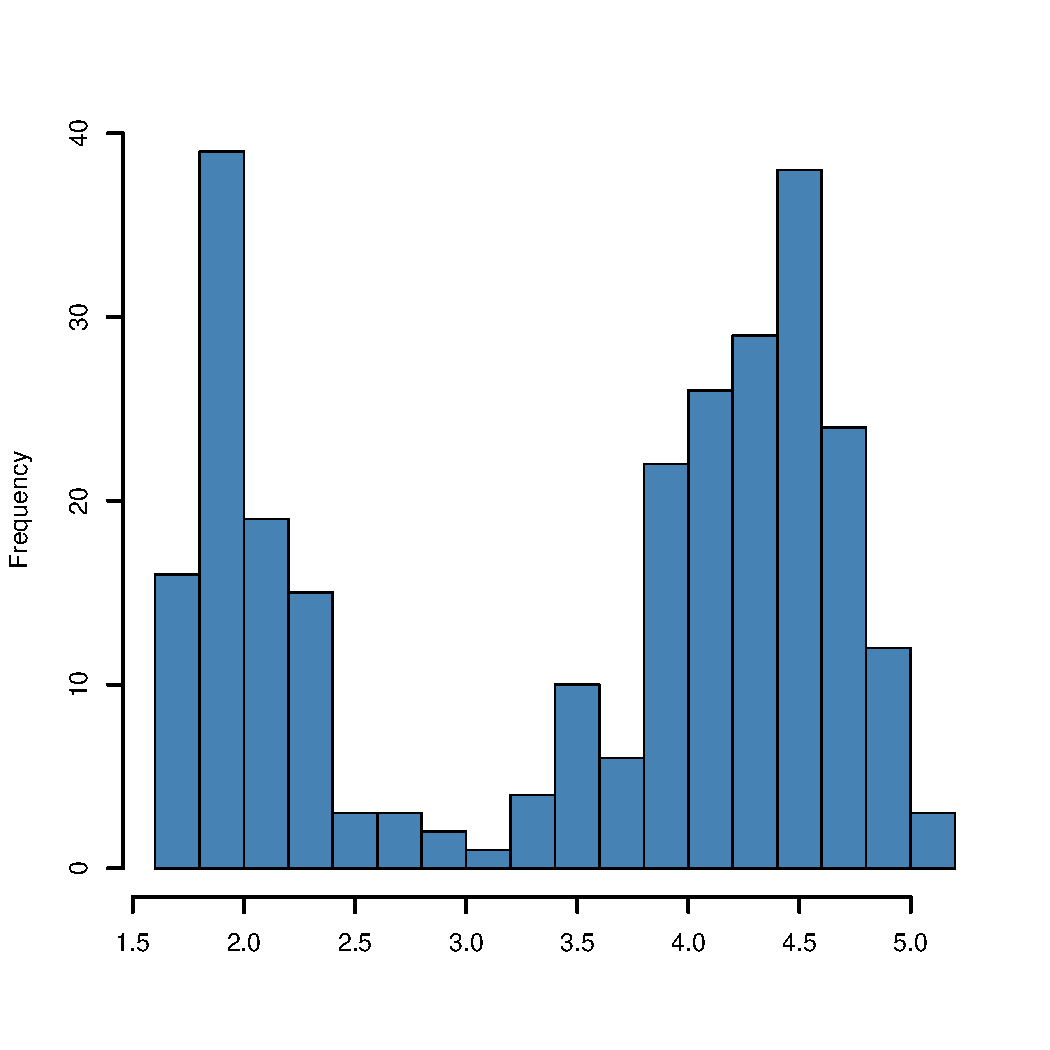
\includegraphics[height=.8\textheight]{img/hist_OlfdFaithful.pdf}
%    \end{figure}
%    \vspace{-.75cm}
%  \end{exampleblock}
%\end{frame}
%
%\begin{frame}{\color{rosee}Bootstrap - IC para la mediana}\small
%  \begin{exampleblock}{Old Faithful dataset}
%    Los pasos son
%    \begin{enumerate}
%    \item Datos: $x_1, x_2, \dots, x_{272}$.
%    \item Mediana: $x_{mediana} = 4$.
%    \item Buscamos $x^*_{mediana}$ de una muestra bootstrap
%      $x_1^*, x_2^*, \dots, x_{272}^*$. Repetimos $1000$ veces.
%    \item Calculamos las diferencias:
%      $\delta^* = x_{mediana}^*-x_{mediana}$.
%    \item Buscamos los valores $\delta_{0.95}^*$ y $\delta_{0.05}^*$.
%    \end{enumerate}
%    El intervalo de confianza bootstrap de nivel $90\%$ obtenido es:
%    \[IC_{mediana} = [3.917; 4.167]\]
%  \end{exampleblock}
%\end{frame}
%
%\begin{frame}{\color{rosee}Bootstrap - IC para la mediana}\small
%  \begin{exampleblock}{Old Faithful dataset}
%    \begin{figure}
%      \centering
%      \subfigure{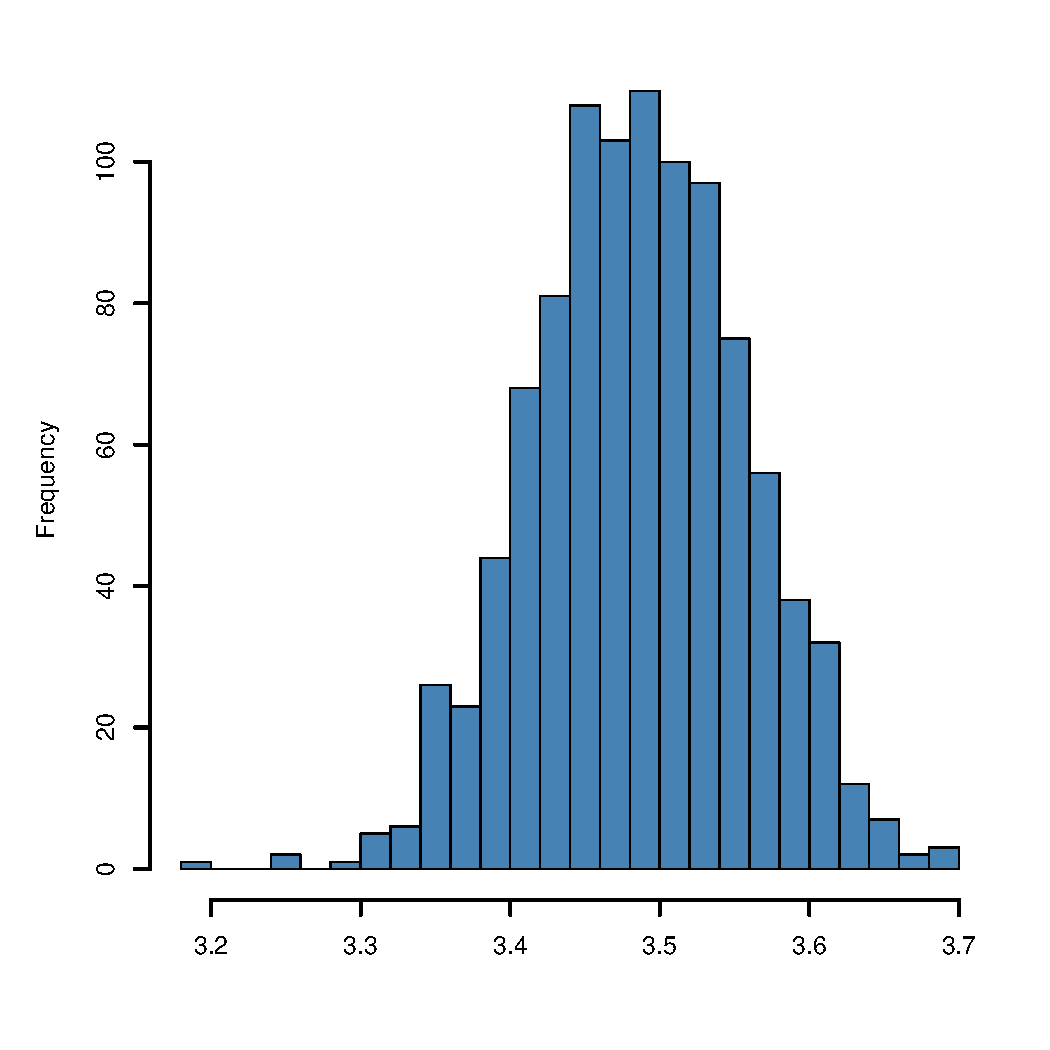
\includegraphics[width=.45\textwidth]{img/hist_OlfdFaithful-means-boot.pdf}}
%      \subfigure{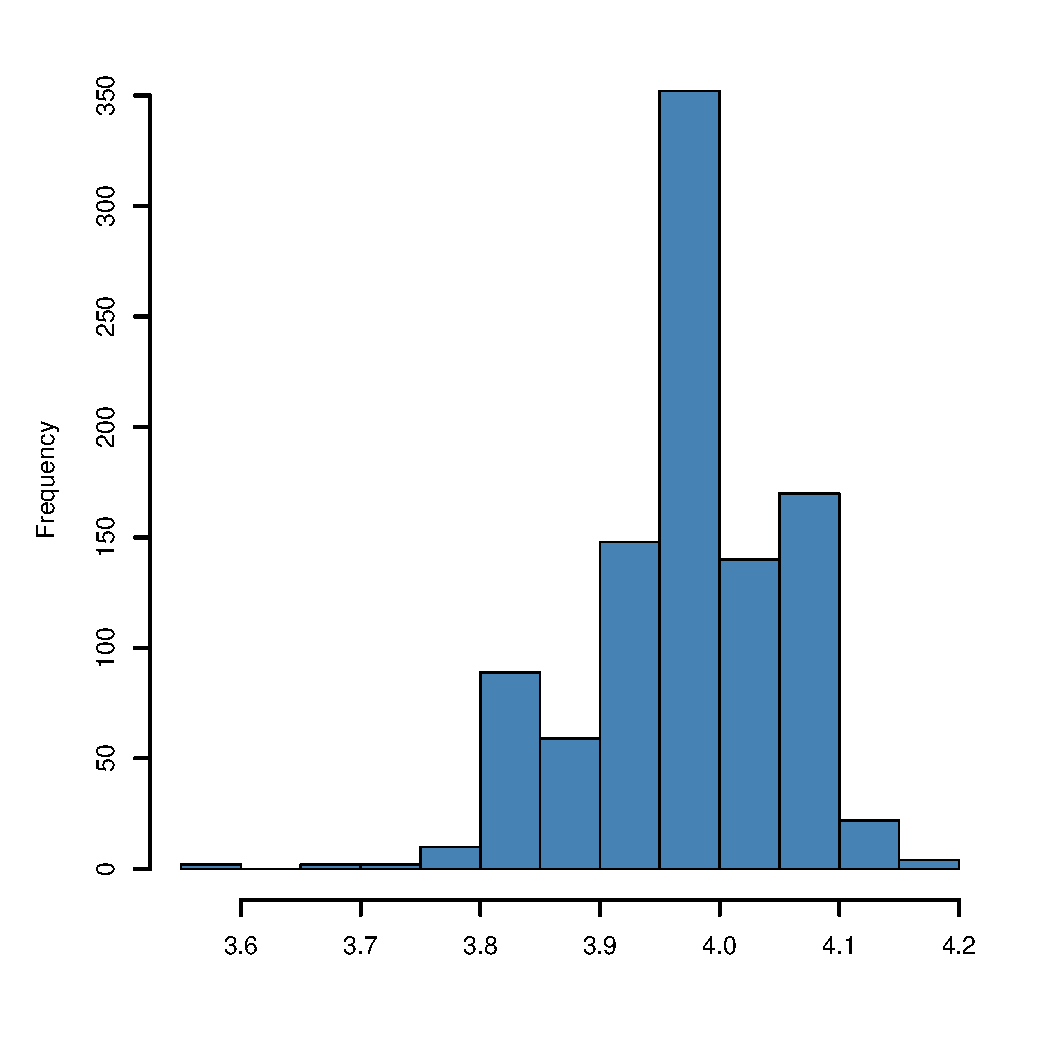
\includegraphics[width=.45\textwidth]{img/hist_OlfdFaithful-medians-boot.pdf}}
%      \end{figure}
%  \end{exampleblock}
%\end{frame}
%
%\begin{frame}{\color{rosee}Bootstrap - IC para la mediana}\small
%  \begin{exampleblock}{Old Faithful dataset}
%    Si en vez de estimar la mediana quisi\'eramos estimar
%    \[P(|\overline{X}_{n}-\mu| > 5) \] procedemos de la misma manera pero
%    calculando la media muestral:
%    \begin{enumerate}
%    \item Datos: $x_1, x_2, \dots, x_{272}$.
%    \item Media muestral: $\overline{x} = 4$.
%    \item Calculamos $\overline{x}^*$ para $1000$ muestras
%      bootstrap $x_1^*, x_2^*, \dots, x_{272}^*$.
%    \item Calculamos las diferencias:
%      $\delta^* = \overline{x}^*-\overline{x}$.
%    \item Usamos la distribuci\'on de $\delta^*$ para aproximar la de
%      $\Delta = \overline{X}_{n}-\mu$:
%      \[P(|\overline{X}_{n}-\mu| >5) = P(|\Delta| > 5) \approx P(|\delta^*|
%        > 5) = 0.225\]
%    \end{enumerate}
%  \end{exampleblock}
%\end{frame}

%\begin{frame}{\color{rosee}Intervalos de confianza por Thecbychev}
  
% \end{frame}
\end{document}





\begin{comment}
    \begin{tikzpicture}[scale=0.4]
\begin{axis}[
  no markers, 
  domain=-7:7, 
  samples=100,
  ymin=0,
  axis lines*=left, 
  xlabel=$\bar{x}$,
  every axis y label/.style={at=(current axis.above origin),anchor=south},
  every axis x label/.style={at=(current axis.right of origin),anchor=west},
  height=5cm, 
  width=15cm,
  xtick=\empty, 
  ytick=\empty,
  enlargelimits=false, 
  clip=false, 
  axis on top,
  grid = major,
  hide y axis
  ]

\pgfmathsetmacro\valueA{gauss(2,4,1)}
\pgfmathsetmacro\valueB{gauss(4,4,1)}
\pgfmathsetmacro\valueC{gauss(0.3,0.3,1)}

%\draw [thick, gray, fill opacity=0.1]  (axis cs:4,0) -- (axis cs:4,\valueB);
\addplot [very thick,cyan!50!black] {gauss(x, 0.3, 1)};
\addplot [fill=cyan!50, draw=none, domain=2:7] {gauss(x,0.3,1)} \closedcycle;

\addplot [very thick,cyan!50!black] {gauss(x, 4, 1)};
\draw [thick, gray, fill opacity=0.1]  (axis cs:2,0) -- (axis cs:2,\valueA);
\draw [thick, gray, fill opacity=0.1]  (axis cs:0.3,0) -- (axis cs:0.3,\valueC);

\draw [yshift=1cm, latex-latex](axis cs:-7, 0) -- node [fill=white] {$1- \beta = 0.9987$} (axis cs:2, 0);
\draw [yshift=1cm, latex-latex](axis cs:2, 0) -- node [fill=white] {$\beta = 0.0013$} (axis cs:6, 0);

\draw [yshift=1cm, latex-latex](axis cs:-7, -0.2) -- node [fill=white] {R $H_0$} (axis cs:2, -0.2);
\draw [yshift=1cm, latex-latex](axis cs:2, -0.2) -- node [fill=white] {NR $H_0$} (axis cs:7, -0.2);

\node[below] at (axis cs:2, 0)  {$\bar{x}_c=776$};
\node[below] at (axis cs:4, 0)  {$\mu_0=800$}; 
\node[below] at (axis cs:0.3, 0)  {$\mu_v=740$}; 
\end{axis}
\end{tikzpicture}
\end{comment}

% \begin{frame}[fragile]{¿Si la muestra no es normal??}
%   Supongamos ahora que $X_i \sim Poisson(3)$ para $i=1,\ldots,10$.
%   \begin{lstlisting}
%     #parametros
%     nreps = 10000
%     mu = 3
%     n = 10
%     alfa = 0.05
%     
%     #intervalos
%     for (i in 1:nreps) {
%     X = rpois(n,mu)
%     linf[i] = mean(X) - qt(1-alfa/2, n-1)*sd(X)/sqrt(n)
%     lsup[i] = mean(X) + qt(1-alfa/2, n-1)*sd(X)/sqrt(n)
%   }
%     
%     # calculamos la proporcion de veces el IC contiene a mu
%     sum(mu<lsup & mu>linf)/nreps
%   \end{lstlisting}
% \end{frame}

% \begin{frame}[fragile]{Ejercicios}
%   Ejercicio: Se registr\'o el contenido de \'acido sulf\'urico de 7
%   contenedores similares obteni\'endose los siguientes
%   $$9.8, 10.2, 10.4, 9.8, 10.0, 10.2, 9.6$$
%   Encuentre un IC del 95\% para $\mu$, la media de
%   todos los contenedores, si se supone una distribuci\'on aproximadamente normal.

%   Ejercicio: Se registr\'o el tiempo de secado, en hora, de cierta marca
%   de pintura latex obteni\'endose los siguientes tiempos:
%   $$    3.4, 2.5, 4.8, 2.9, 3.6, 2.8, 3.3, 5.6,
%   3.7, 2.8, 4.4, 4.0, 5.2, 3.0, 4.8$$ Encuentre un IC del 95\% y uno del
%   99\% para $\mu$, la media de tiempo de secado, si se supone una
%   distribuci\'on aproximadamente normal.
% \end{frame}

% \begin{frame}[fragile]{?`Se puede hacer esto directamente en R?}

%     La respuesta es SI! Investigar la funci\'on \verb't.test'

%    \small{
%         \begin{verbatim}
%         x = c(3.4, 2.5, 4.8, 2.9, 3.6, 2.8, 3.3, 5.6, 3.7,
%         2.8, 4.4, 4.0, 5.2, 3.0, 4.8)

%         t.test(x)
%         One Sample t-test
%         data:  x
%         t = 15.1051, df = 14, p-value = 4.64e-10
%         alternative hypothesis: true mean is not equal to 0
%         95 percent confidence interval:
%         3.248995 4.324339
%         sample estimates:
%         mean of x
%         3.786667
%         \end{verbatim}

%      \textcolor{dodgerblue}{Atenci\'on! Esto se puede hacer si tenemos la
%        muestra, pero si \'unicamente tenemos el valor de la media y la
%        varianza muestral no es posible utilizarlo.}}
% \end{frame}

% % 
% \begin{frame}
% Ejercicio 9.13
% \end{frame}
%
%\begin{frame}{\color{rosee}?`Qu\'e forma tiene un IC para la media $\mu$?}
%
%\bigskip
%
%Si la varianza es conocida:
%
%\[ \left( \overline{X}_{n} - A \sqrt{ {\hbox{var} (\overline{X}_{n})}} , \overline{X}_{n} + A \sqrt{ {\hbox{var} (\overline{X}_{n})}} \right)\]
%donde $A$ es una $z$.
%
%\pause
%Si la varianza es desconocida
%
%\[ \left( \overline{X}_{n} - A \sqrt{ {\widehat{\hbox{var}} (\overline{X}_{n})}} , \overline{X}_{n} +A \sqrt{ \widehat{ \hbox{var}} (\overline{X}_{n})}\right) \]
%
%
%donde $A$ es una $t$.
%\end{frame}
%
%\begin{frame}{\color{rosee}En general, ?`qu\'e forma tiene un IC para un par\'ametro?}
%
%  Cuando quiero un intervalod e confianza para un parametro $\theta$ es
%  de la forma (cuando la varianza del estimador de $\theta$ es
%  conocida:
%  \[ \left( \widehat{\theta} - A \sqrt{ {\hbox{var} (\widehat{\theta}
%      )}} , \widehat{\theta} +A\sqrt{ {\hbox{var} (\widehat{\theta} )}}
%    \right) \]

%y si la varianza es desconocida
%
%\[ \left( \widehat{\theta} - A\sqrt{ \widehat{\hbox{var}}
%    (\widehat{\theta}) } , \widehat{\theta} + A \sqrt{
%    \widehat{\hbox{var}}( \widehat{\theta}) } \right)\]
%
%\end{frame}

\begin{frame}{\color{rosee}Intervalos de confianza} \small

  Si el nivel de confianza es alto y el intervalo resultante es angosto,
  nuestro conocimiento sobre el par\'ametro es razonablemente preciso.

  Un intervalo de confianza ancho, indica un alto nivel de incertidumbre
  sobre el valor estimado.
\end{frame}

\begin{frame}{\color{rosee}Intervalos de confianza} \small

  Supongamos que $X \sim N(\mu,\sigma^2)$ con $\mu$
  desconocida y $\sigma^2$ conocida.
  \[Z = \frac{\overline{X}_{n}-\mu}{\sigma/\sqrt{n}} \sim N(0,1)\]
  Llamemos $z_{\alpha}$ al valor que verifica:
  \[P(Z < z_{\alpha}) = \alpha\]
  Entonces sabemos que
  \[P(-z_{1-\frac{\alpha}{2}} < Z < z_{1-\frac{\alpha}{2}}) = \alpha\]
  Despejando
  \[P \left(\underbrace{\overline{X}_{n}-z_{1-\frac{\alpha}{2}}
        \frac{\sigma}{\sqrt{n}} < \mu < \overline{X}_{n} + z_{1-\frac{\alpha}{2}}
        \frac{\sigma}{\sqrt{n}}}_{\mbox{intervalo aleatorio}}\right) =
    \alpha\]
\end{frame}

\begin{frame}{\color{rosee}Intervalos de confianza} \small
  Observemos que el intervalo es aleatorio pero su ancho no lo es:
  \[2 \cdot z_{1-\frac{\alpha}{2}} \frac{\sigma}{\sqrt{n}}\] solo su punto central
  $\overline{X}_{n}$.
\end{frame}

\begin{frame}{\color{rosee}no conozco $\sigma$}
  
\end{frame}

% * basados en maxima verosimilitud

\begin{frame}{\color{rosee}Ejemplo}
  % A finite mathematics course has recently been changed, and the
  % homework is now done online via computer instead of from the textbook
  % exercises. How can we see if there has been improvement? Past
  % experience suggests that the distribution of final exam scores is
  % normally distributed with mean 65 and estándar deviation 13. It is
  % believed that the distribution is still normal with estándar deviation
  % 13, but the mean has likely changed. A sample of 40 students has a
  % mean final exam score of 70.7. Let’s calculate a confidence interval
  % for the population mean using a confi- dence level of
  % 90%. This requires that 100(1  a) 1⁄4 90, from which a 1⁄4 .10 and
  % z a/2 1⁄4 z .05 1⁄4 1.645 (corresponding to a cumulative z-curve area
  % of .9500).  The desired interval is then 13 70:7  1:645  p
  % ffiffiffiffiffi 1⁄4 70:7  3:4 1⁄4 ð67:3; 74:1Þ 40 With a reasonably
  % high degree of confidence, we can say that 67.3 < m < 74.1.
  % Furthermore, we are confident that the population mean has improved
  % over the ■ previous value of 65.
\end{frame}

\begin{frame}{\color{rosee}En general}
  
\end{frame}
\end{document}